% TOO BUSY?
\documentclass[10pt]{beamer}
\usepackage{verbatim}
\usepackage{wasysym}
\usepackage{tikzsymbols}
\input{header.tex}

%\title{Evolutionary inference reveals mtDNA gene retention dependence on hydrophobicity, GC content, and control of complex assembly}
\title{Statistics and model selection: Doing science with data}
\institute{\vspace{-0.8cm} \\ \large Iain Johnston \vspace{0.25cm} \\  \includegraphics[width=0.025\textwidth]{twitter.png} \footnotesize @mitomaths \\ \scriptsize Department of Mathematics\\ University of Bergen\\ \vspace{0.4cm}} %\includegraphics[width=0.6\textwidth]{funders.png} }
\date{}
%\date{}

\renewcommand{\cellsys}{\mycite{Cell Systems \textbf{2} 101 (2016)}}
\newcommand{\cellsystwo}{\mycite{Cell Systems \textbf{13} e5 (2022)}}
\newcommand{\casali}{\mycite{Casali et al., Nat Genet \textbf{46} 279 (2014)}}
\newcommand{\marcus}{\mycite{Bioinformatics \textbf{39} btac803 (2023)}}
\newcommand{\hypertraps}{\mycite{Cell Systems \textbf{10} 39 (2020)}}
\newcommand{\jallow}{\mycite{Jallow et al. PLoS ONE \textbf{7} e45645 (2012)}}
\newcommand{\malaria}{\mycite{npj Digital Medicine \textbf{2} 63 (2019)}}

\begin{document}

\frame{\titlepage}

\begin{frame}{(Philosophical?) Introduction}
  \begin{itemize}
  \item Statistics is \textbf{not} the discipline of looking up vast tables of numbers in decades-old textbooks
  \item Statistics is \textbf{how we connect our scientific ideas to the world around us}!
  \end{itemize}
  \begin{columns}
    \begin{column}{0.45\textwidth}
      \begin{itemize}
  \item Stats makes discoveries
  \item Stats gives us amazing ways to deal with the universe's messiness
  \item Stats predicts the future
  \item Stats is central to the scientific method
    \end{itemize}
  \end{column}
  \begin{column}{0.55\textwidth}
    \includegraphics[width=1\textwidth]{biostats-umiami.jpeg} 
    \figcred{U of Miami}
  \end{column}
  \end{columns}
\end{frame}

\section{Is modelling science?}

\begin{frame}{Are we `scientists'?}
\includegraphics[width=.6\textwidth]{method.jpg} \\
\figcred{bigpicturebiology.com}
\end{frame}
\begin{frame}{Are we `scientists'?}
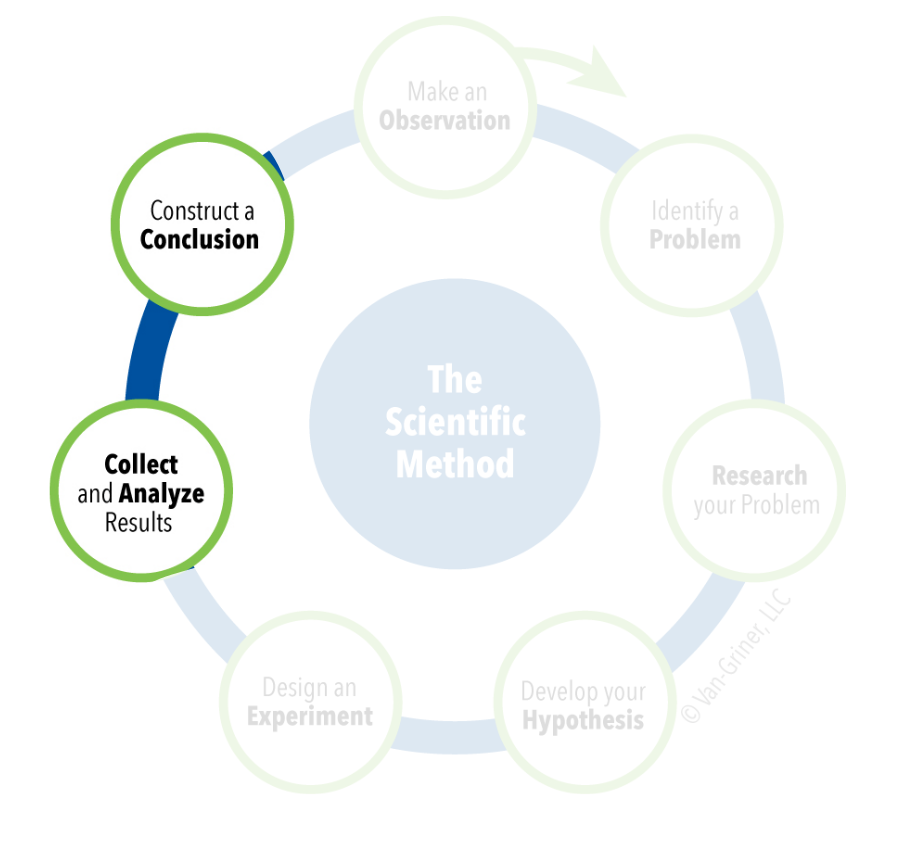
\includegraphics[width=.6\textwidth]{method-1.png} \\
\figcred{bigpicturebiology.com}
\end{frame}
\begin{frame}{Are we `scientists'?}
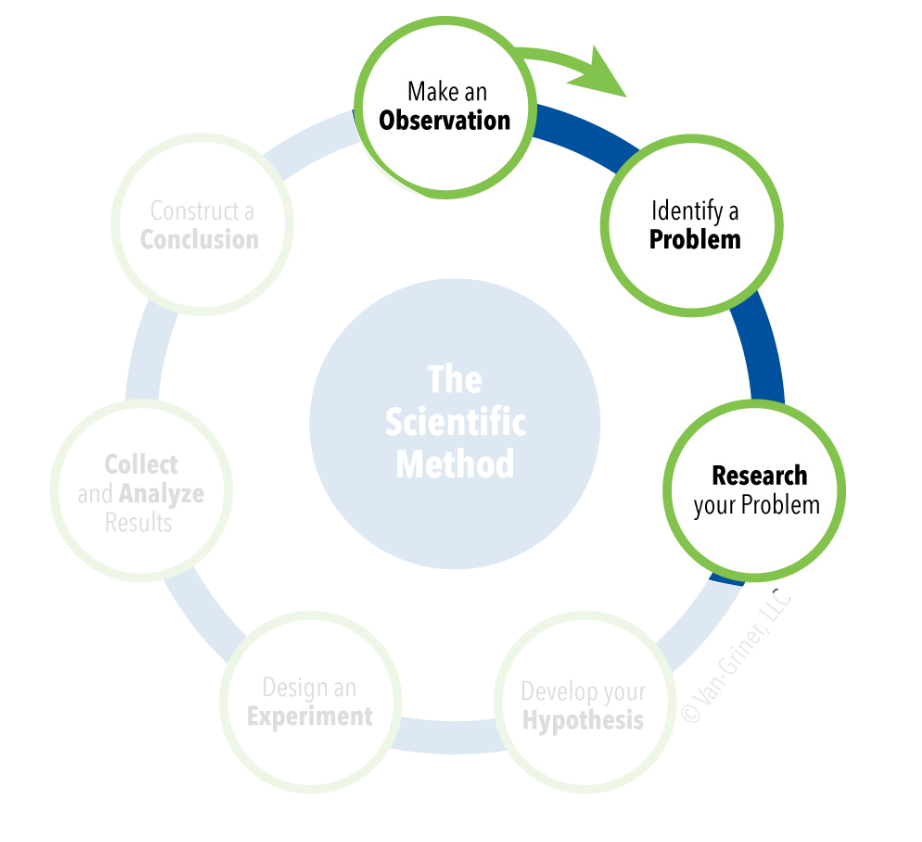
\includegraphics[width=.6\textwidth]{method-2.png} \\
\figcred{bigpicturebiology.com}
\end{frame}
\begin{frame}{Are we `scientists'?}
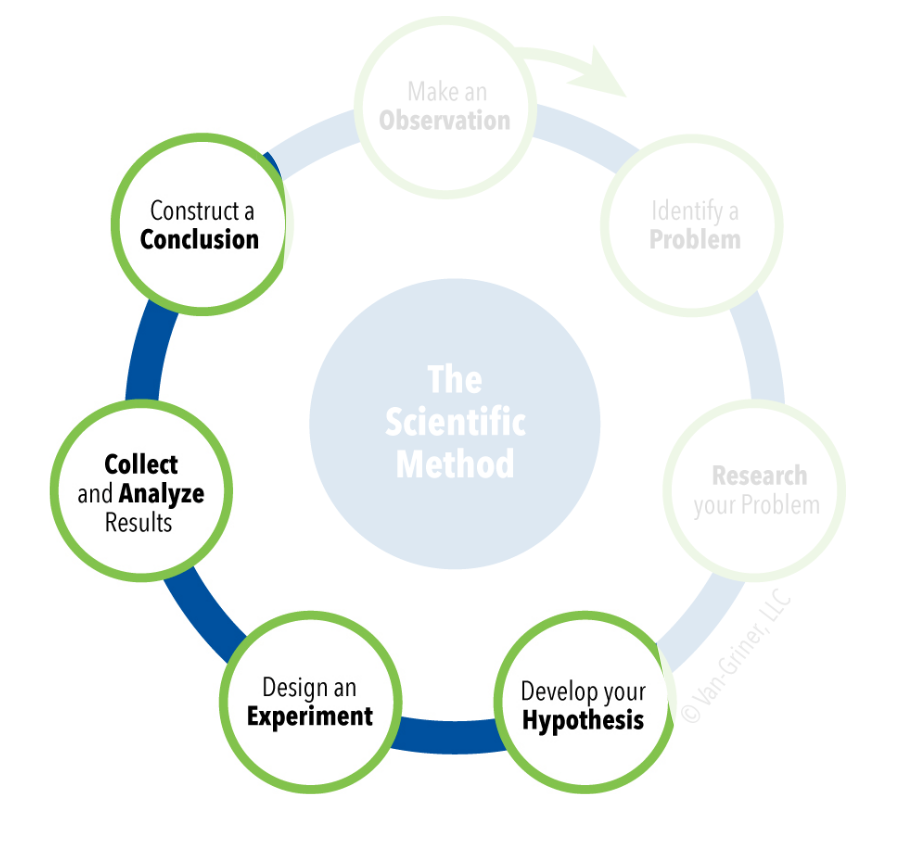
\includegraphics[width=.6\textwidth]{method-3.png} \\
\figcred{bigpicturebiology.com}
\end{frame}


\begin{frame}{What is data science?}
   Applying science to data? \figcred{Cao \& Gao, Nature Biotech 2022} \\
  \includegraphics[width=.55\textwidth]{science-data.png} 
  
 
  Doing science with data? \figcred{Thorne \& Stumpf, J Roy Soc Interf 2012} \\
  \includegraphics[width=.6\textwidth]{data-science.png} 
  
  \end{frame}

\begin{frame}{Is modelling science?}
  \begin{columns}
    \begin{column}{0.4\textwidth}
  \begin{itemize}
  \item Build a statistical / physical / computational model
  \item It fits data better than a null model
    \item Maybe it predicts some new data better than a null model
    \item Publish?
  \end{itemize}
    \end{column}
    \begin{column}{0.6\textwidth}
    \end{column}
        \end{columns}
\end{frame}
\begin{frame}{Is modelling science?}
  \begin{columns}
    \begin{column}{0.4\textwidth}
  \begin{itemize}
  \item Build a statistical / physical / computational model
  \item It fits data better than a null model
    \item Maybe it predicts some new data better than a null model
    \item Publish?
      \item ... could we have done better?
  \end{itemize}
    \end{column}
    \begin{column}{0.6\textwidth}
    \end{column}
        \end{columns}
\end{frame}
\begin{frame}{Is modelling science?}
  \begin{columns}
    \begin{column}{0.4\textwidth}
  \begin{itemize}
  \item Build a statistical / physical / computational model
  \item It fits data better than a null model
    \item Maybe it predicts some new data better than a null model
    \item Publish?
      \item ... could we have done better?
  \end{itemize}
    \end{column}
    \begin{column}{0.6\textwidth}
      \includegraphics[width=\textwidth]{medallist.jpg}
      \figcred{3palec}
    \end{column}
        \end{columns}
\end{frame}

\begin{frame}{Is modelling science?}
  \begin{columns}
    \begin{column}{0.4\textwidth}
  \begin{itemize}
  \item Build a statistical / physical / computational model
  \item It fits data better than a null model
    \item Maybe it predicts some new data better than a null model
    \item Publish?
      \item ... could we have done better?
  \end{itemize}
    \end{column}
    \begin{column}{0.6\textwidth}
   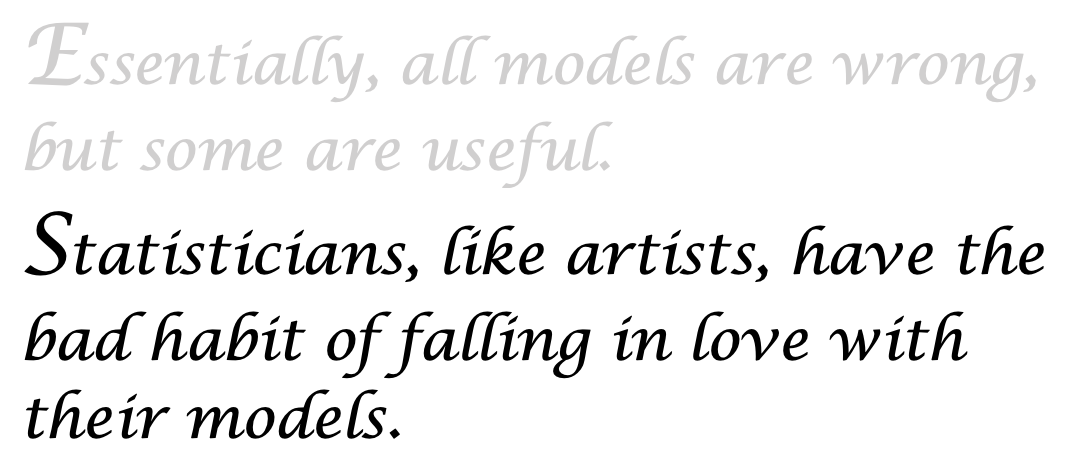
\includegraphics[width=\textwidth]{boxquote.png}
    - George Box
    \end{column}
        \end{columns}
\end{frame}


\begin{frame}{Model selection}
  Which model is best?
  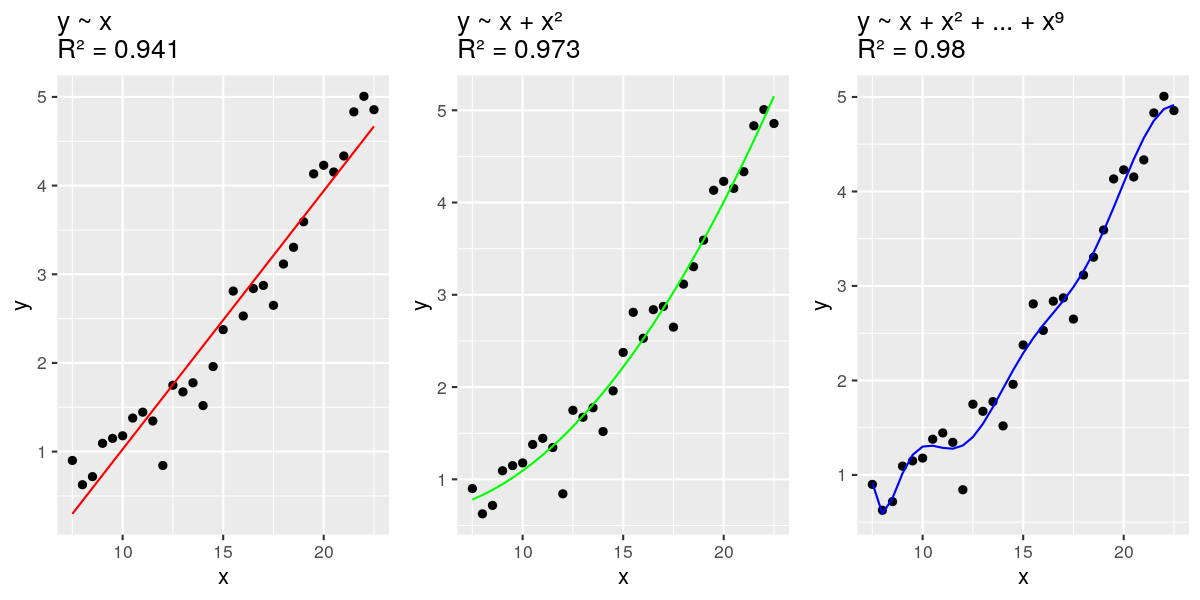
\includegraphics[width=\textwidth]{cedas-model-1.png}
\end{frame}

\begin{frame}{Model selection}
  Which model is best?
  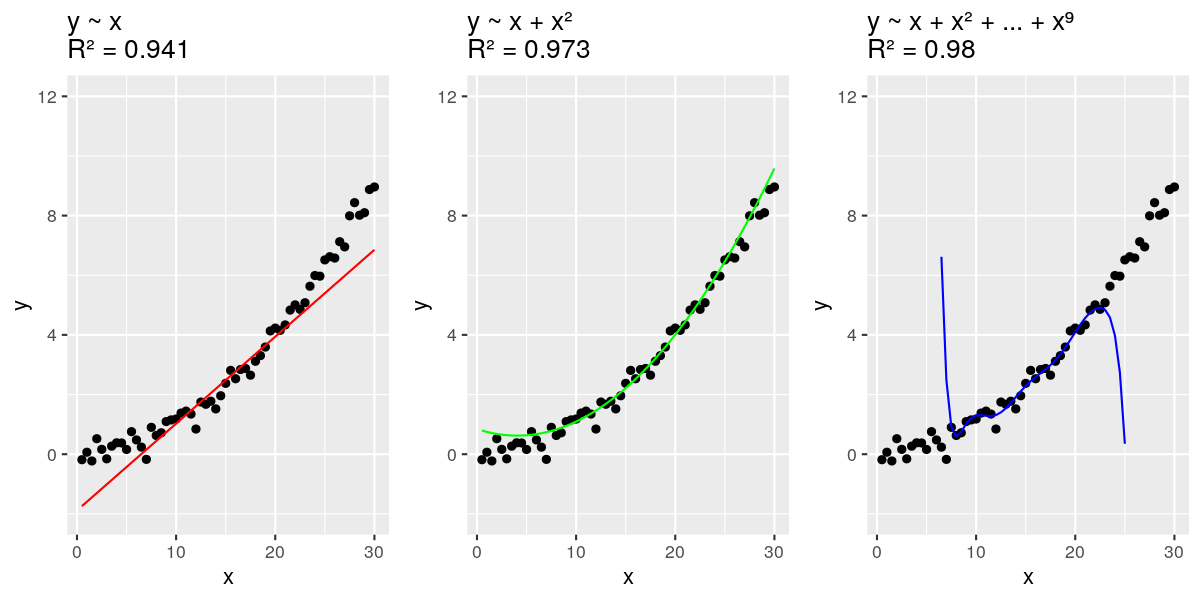
\includegraphics[width=\textwidth]{cedas-model-2.png}
\end{frame}

\begin{frame}{Models in the sciences}
  \begin{itemize}
   \item Statistical models are mathematical representations of a (wrong) theory about the real world
   \item They describe a \textbf{probability distribution} $P(Y|\textcolor{red}{\theta})$ from which observations $y$ are drawn
   \item \textbf{Parameters} $\textcolor{red}{\theta}$ of a model control this probability distribution
  \end{itemize}
  \centering
      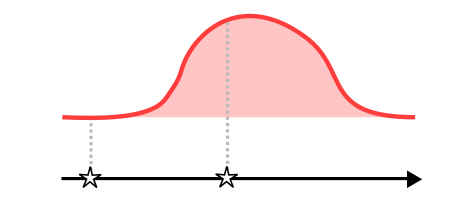
\includegraphics[width=.8\textwidth]{camria-prob-3.png}
\end{frame}
\begin{frame}{Models in the sciences}
  \begin{itemize}
   \item Statistical models are mathematical representations of a (wrong) theory about the real world
   \item They describe a \textbf{probability distribution} $P(Y|\textcolor{blue}{\theta})$ from which observations $y$ are drawn
   \item \textbf{Parameters} $\textcolor{blue}{\theta}$ of a model control this probability distribution
  \end{itemize}
  \centering
      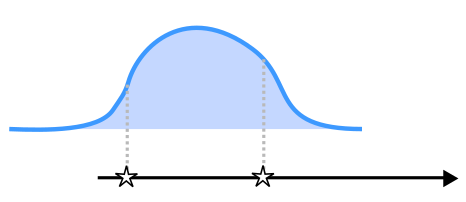
\includegraphics[width=.8\textwidth]{camria-prob-4.png}
\end{frame}
\begin{frame}{Models in the sciences}
  \begin{itemize}
   \item Statistical models are mathematical representations of a (wrong) theory about the real world
   \item They describe a \textbf{probability distribution} $P(Y|\textcolor{green}{\theta})$ from which observations $y$ are drawn
   \item \textbf{Parameters} $\textcolor{green}{\theta}$ of a model control this probability distribution
  \end{itemize}
  \centering
      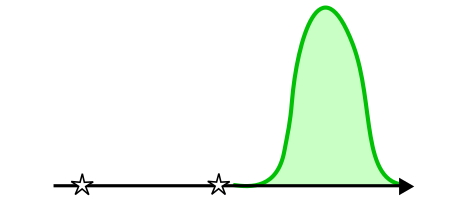
\includegraphics[width=.8\textwidth]{camria-prob-5.png}
\end{frame}





\begin{frame}{Models in the sciences}
  \begin{columns}
    \begin{column}{0.34\textwidth}
  \begin{itemize}
  \item Probability of all observations together given some parameters $=$ \textbf{likelihood} for those parameters
    \item $\prod_i P(y_i | \theta) = \mathcal{L}(\theta)$
    \item Likelihood behaves very much like a goodness-of-fit
      \item $\mathcal{L}(\textcolor{blue}{\theta}) > \mathcal{L}(\textcolor{green}{\theta})$
  \end{itemize}
    \end{column}
    \begin{column}{0.65\textwidth}
          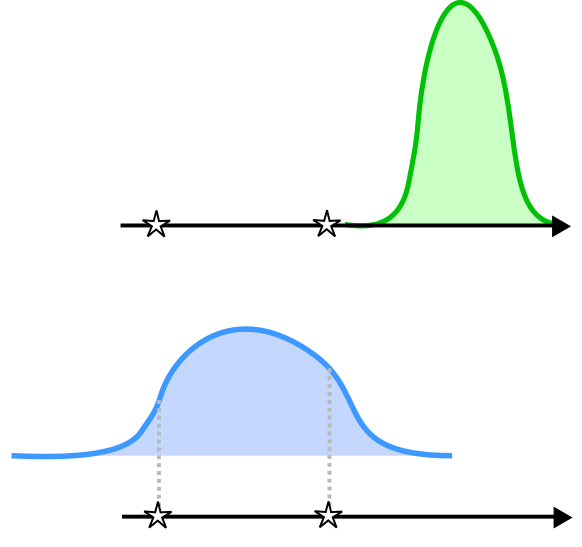
\includegraphics[width=\textwidth]{camria-lik.png}
    \end{column}
        \end{columns}
\end{frame}

\begin{frame}{Models in the sciences}
  \begin{columns}
    \begin{column}{0.34\textwidth}
  \begin{itemize}
  \item Maximising likelihood: find parameter set $\hat{\theta}$ most likely to generate our observations
    \item $\textcolor{blue}{\theta}$ will be closer to $\hat{\theta}$ than $\textcolor{green}{\theta}$
  \end{itemize}
    \end{column}
    \begin{column}{0.65\textwidth}
          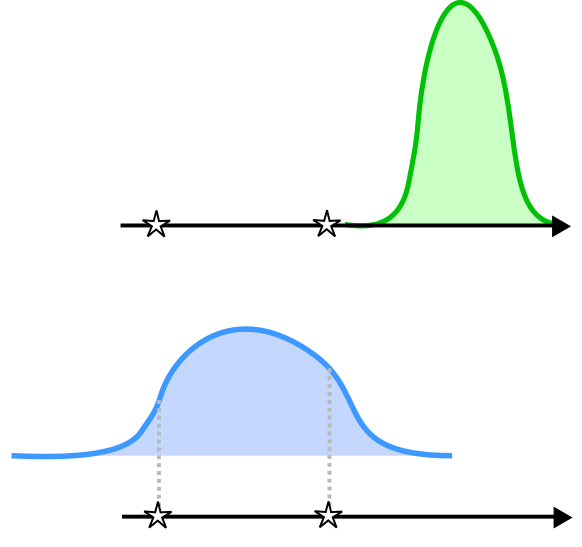
\includegraphics[width=\textwidth]{camria-lik.png}
    \end{column}
        \end{columns}
\end{frame}

\begin{frame}{Model selection}
  Which model is best?
  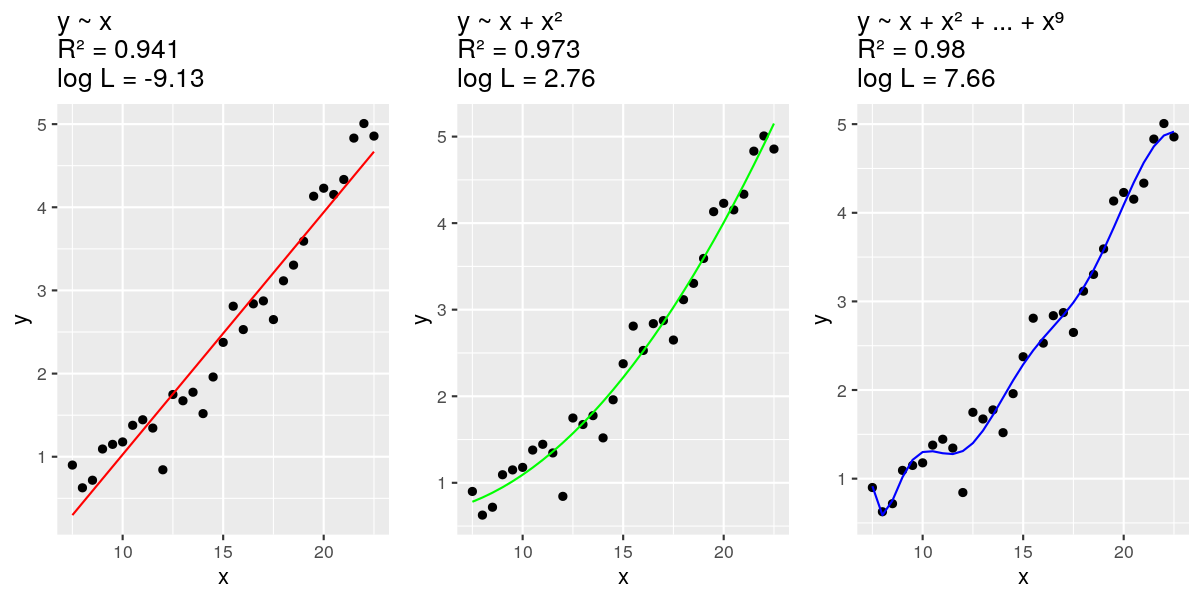
\includegraphics[width=\textwidth]{cedas-model-3.png}
\end{frame}

\begin{frame}{Model selection}
  \begin{itemize}
  \item More complex models (more predictors) will always give a better fit ($R^2, \mathcal{L}$, ...)
  \item They can exploit particular features of the random noise in a system to squeeze closer to datapoints
  \item \textbf{Overfitting} / fitting noise
  \item Simpler models (fewer predictors) have less overfitting risk, but may miss genuine trends in the data (\textbf{underfitting})
  \item We need to \textbf{trade off goodness of fit and complexity}
    \end{itemize}
\end{frame}

\begin{frame}{(One approach for) Frequentist model selection}
  \begin{itemize}
  \item $y$ observations; $\theta$ parameters of a model ($k$ parameters in total)
  \item $\mathcal{L}(\theta) = P(y | \theta)$ likelihood
  \item $\hat{\mathcal{L}} = \mathcal{L}(\hat{\theta}) = \max_{\theta} \mathcal{L}(\theta)$ maximum likelihood
        \item Parameter guess: $\hat{\theta}$ is the single value of $\theta$ at which we get $\hat{\mathcal{L}}$

        \item Akaike Information Criterion:
          \begin{equation*}
            AIC = \underbrace{-2 \log \hat{\mathcal{L}}}_{\text{goodness of fit}} + \underbrace{2k}_{\text{model complexity}}
            \end{equation*}
          \item Low AIC: good fit, low complexity
  \end{itemize}
\end{frame}

\begin{frame}{Model selection with AIC}
  Which model is best?
  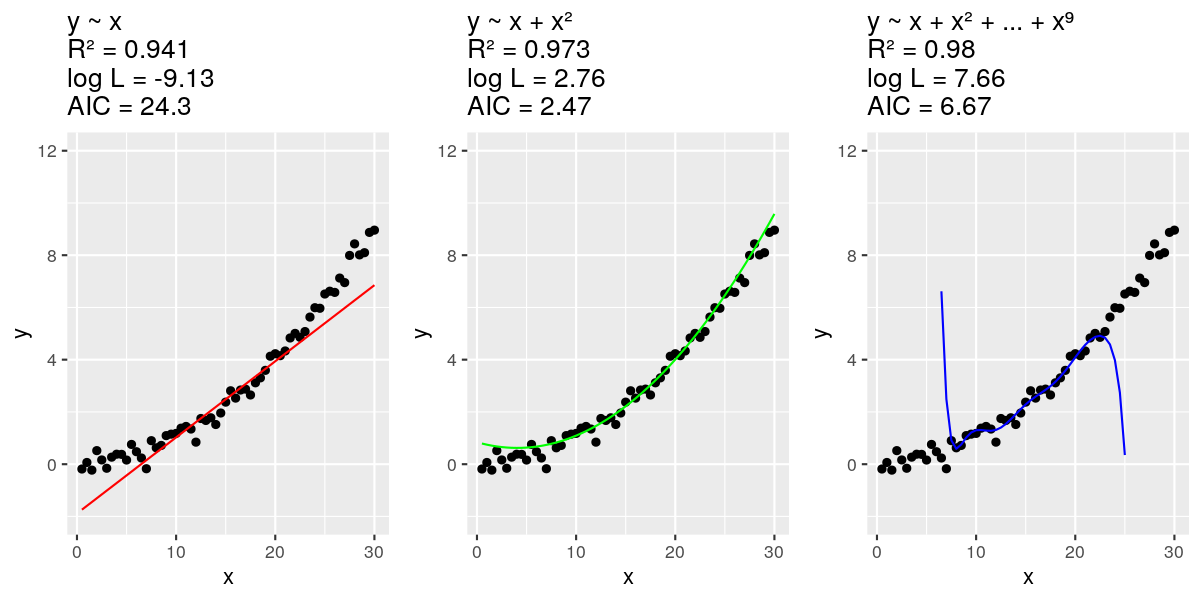
\includegraphics[width=\textwidth]{cedas-model-4.png}
\end{frame}

\begin{frame}{Model selection with AIC}
  \begin{itemize}
        \item $AIC = \underbrace{-2 \log \hat{\mathcal{L}}}_{\text{goodness of fit}} + \underbrace{2k}_{\text{model complexity}}$
        \item AIC gives a tradeoff between goodness of fit and complexity; between overfitting and underfitting
        \item But it only deals with the best possible version of each model -- the one at $\hat{\theta}$
        \item And it only gives us the model that wins, not the probability of different models being true
          \item And it shouldn't be used iteratively \figcred{Flom \& Cassell 2007; Chatfield 1995; Wikipedia page}
  \end{itemize}
\end{frame}

%    \item $P_{posterior}(\theta|y) = \frac{P(y|\theta)}{P(y)} \times P_{prior}(\theta)$
\begin{frame}{Inference using Bayes' rule}
  \begin{itemize}
  \item $y$ observations; $\theta$ parameters of a model
\item[] 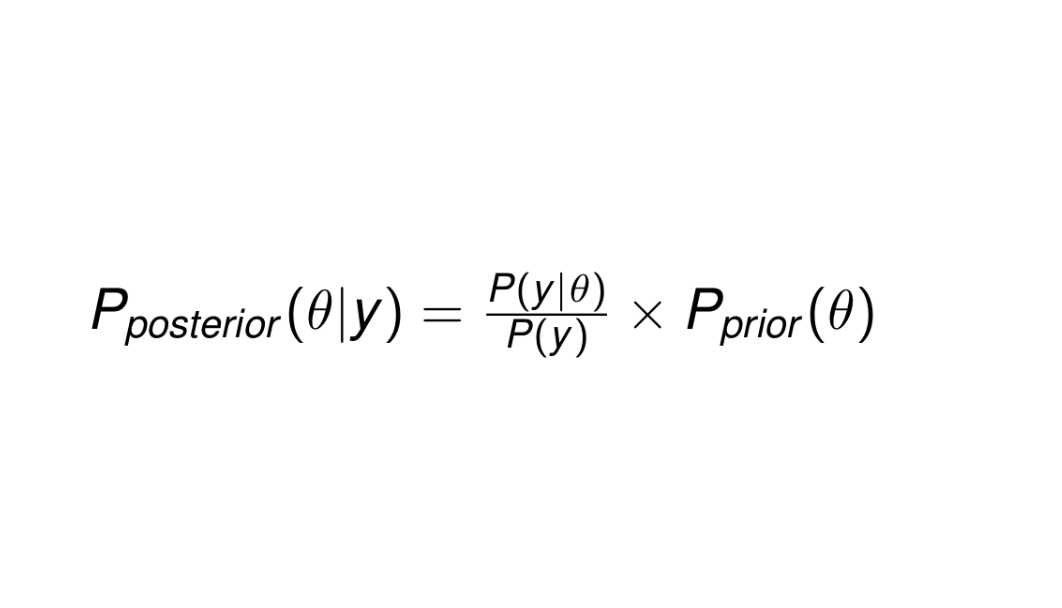
\includegraphics[width=.9\textwidth]{bayes-1.png}
    \item Not a single value, but a distribution of possible $\theta$ values
  \end{itemize}
\end{frame}
\begin{frame}{Inference using Bayes' rule}
  \begin{itemize}
  \item $y$ observations; $\theta$ parameters of a model
\item[] 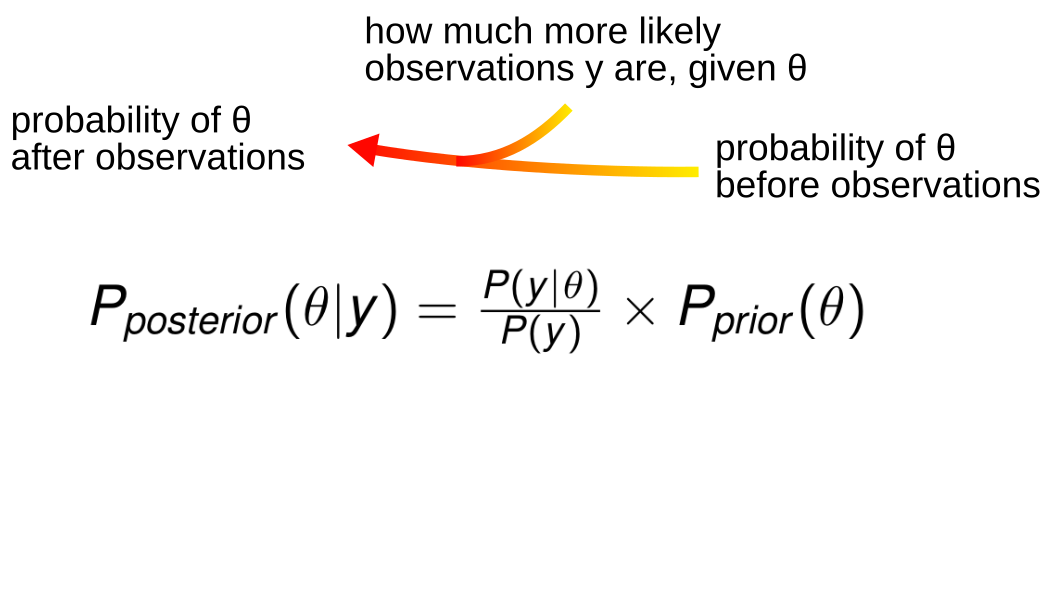
\includegraphics[width=.9\textwidth]{bayes-2.png}
    \item Not a single value, but a distribution of possible $\theta$ values
  \end{itemize}
\end{frame}
\begin{frame}{Inference using Bayes' rule}
  \begin{itemize}
  \item $y$ observations; $\theta$ parameters of a model
\item[] 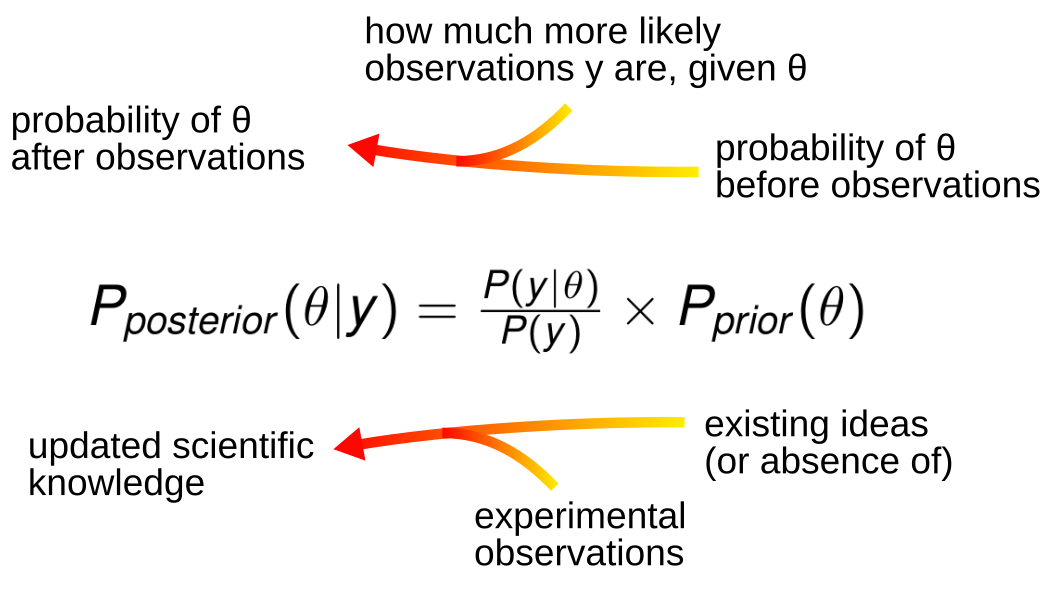
\includegraphics[width=.9\textwidth]{bayes-3.png}
    \item Not a single value, but a distribution of possible $\theta$ values
  \end{itemize}
\end{frame}

\begin{frame}{Inference using Bayes' rule}
  \begin{itemize}
   \item $P_{posterior}(\theta|y) = \frac{P(y|\theta)}{P(y)} \times \textcolor{red}{P_{prior}(\theta)} $
      \end{itemize}
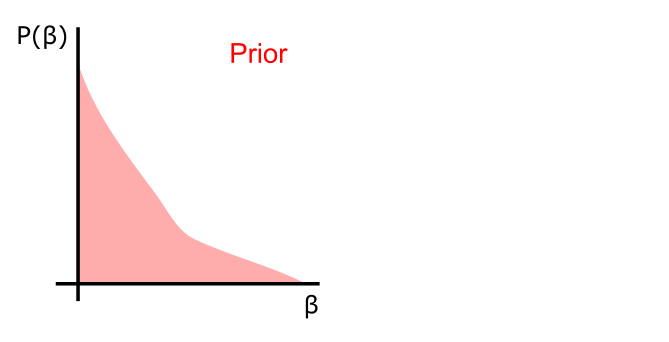
\includegraphics[width=\textwidth]{bayes-inf-1.png}
\end{frame}
\begin{frame}{Inference using Bayes' rule}
  \begin{itemize}
   \item $P_{posterior}(\theta|y) = \frac{P(y|\theta)}{P(y)} \times \textcolor{red}{P_{prior}(\theta)} $
      \end{itemize}
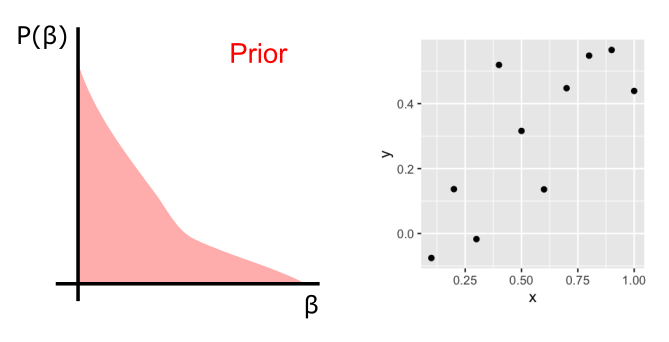
\includegraphics[width=\textwidth]{bayes-inf-2.png}
\end{frame}
\begin{frame}{Inference using Bayes' rule}
  \begin{itemize}
  \item $P_{posterior}(\theta|y) = \textcolor{teal}{\frac{P(y|\theta)}{P(y)}} \times \textcolor{red}{P_{prior}(\theta)} $
      \end{itemize}
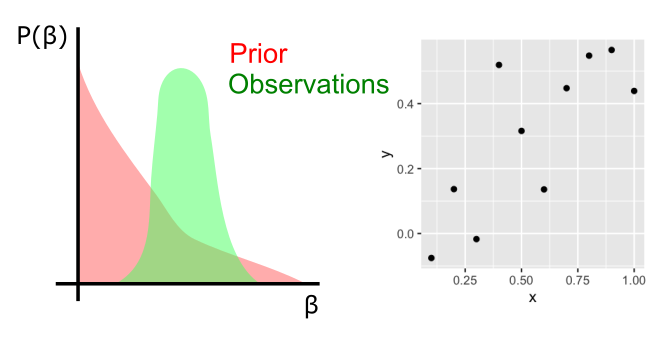
\includegraphics[width=\textwidth]{bayes-inf-3.png}
\end{frame}
\begin{frame}{Inference using Bayes' rule}
  \begin{itemize}
  \item $\textcolor{blue}{P_{posterior}(\theta|y)} = \textcolor{teal}{\frac{P(y|\theta)}{P(y)}} \times \textcolor{red}{P_{prior}(\theta)} $
      \end{itemize}
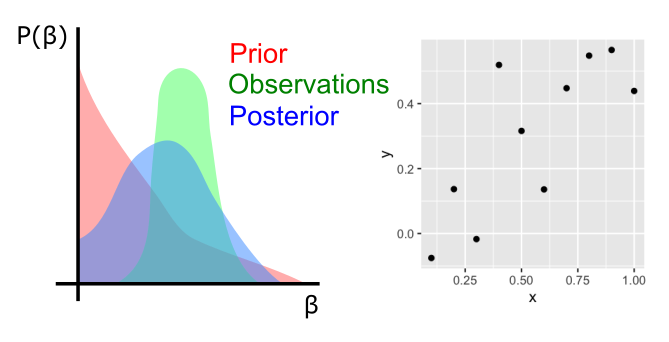
\includegraphics[width=\textwidth]{bayes-inf-4.png}
\end{frame}

\begin{frame}{Bayesian model selection}
  \begin{itemize}
  \item Marginal likelihood $P(y|M) = \int_{\theta} \textcolor{red}{P(y|\theta, M)} \textcolor{gray}{P_{prior}(\theta|M)} d\theta$
  \end{itemize}
  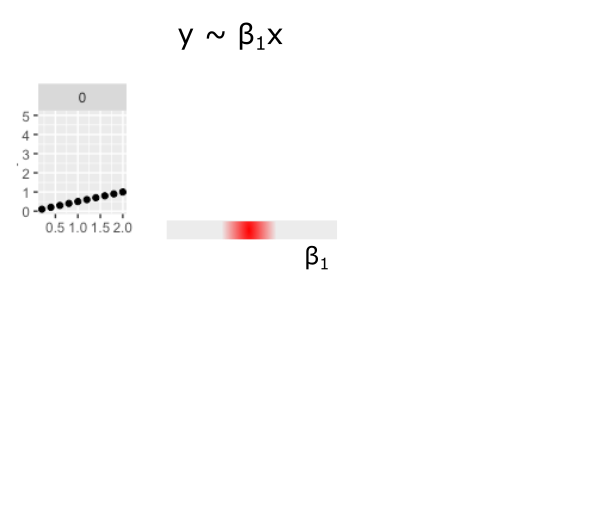
\includegraphics[width=.7\textwidth]{bms-1.png}
\end{frame}
\begin{frame}{Bayesian model selection}
  \begin{itemize}
  \item Marginal likelihood $P(y|M) = \int_{\theta} \textcolor{red}{P(y|\theta, M)} \textcolor{gray}{P_{prior}(\theta|M)} d\theta$
  \end{itemize}
  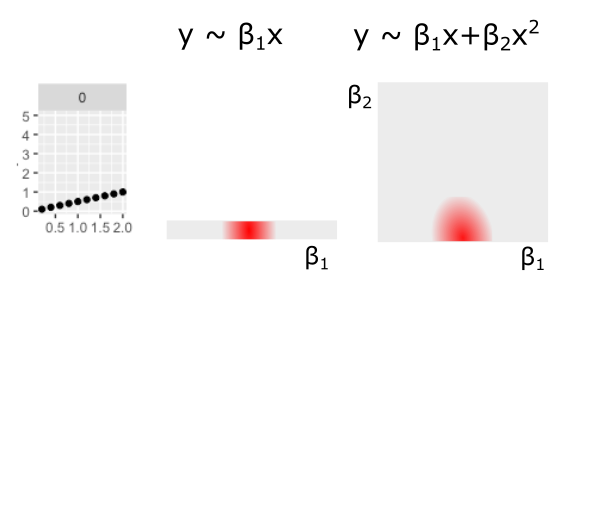
\includegraphics[width=.7\textwidth]{bms-2.png}
\end{frame}
\begin{frame}{Bayesian model selection}
  \begin{itemize}
  \item Marginal likelihood $P(y|M) = \int_{\theta} \textcolor{red}{P(y|\theta, M)} \textcolor{gray}{P_{prior}(\theta|M)} d\theta$
  \end{itemize}
  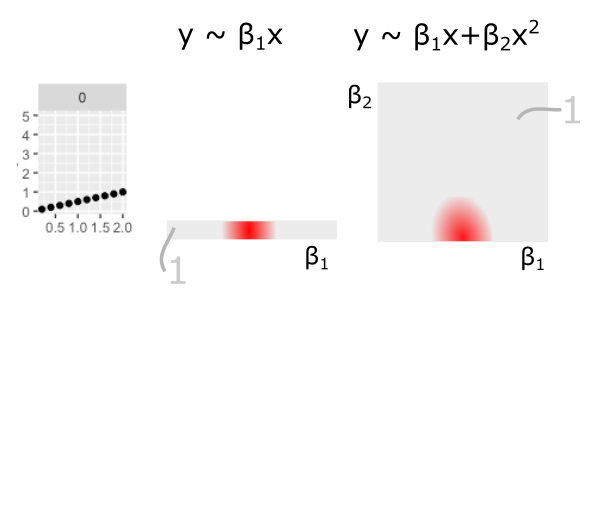
\includegraphics[width=.7\textwidth]{bms-3.png}
\end{frame}
\begin{frame}{Bayesian model selection}
  \begin{itemize}
  \item Marginal likelihood $P(y|M) = \int_{\theta} \textcolor{red}{P(y|\theta, M)} \textcolor{gray}{P_{prior}(\theta|M)} d\theta$
  \end{itemize}
  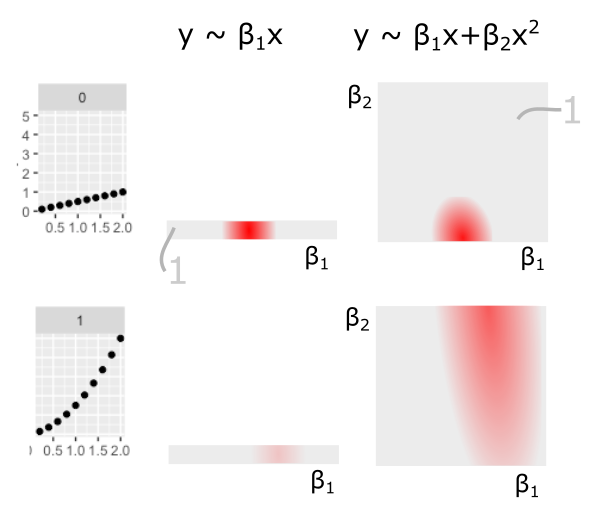
\includegraphics[width=.7\textwidth]{bms-4.png}
\end{frame}

\begin{frame}{Bayesian model selection}
  \begin{itemize}
    \item Marginal likelihood $P(y|M) = \int_{\theta} P(y|\theta, M) P_{prior}(\theta|M) d\theta$
  \end{itemize}
  \includegraphics[width=\textwidth]{cedas-model-sel-x2.png}
  \includegraphics[width=.5\textwidth]{minka.png}
  \figcred{Tom Minka (MIT)}
\end{frame}

\begin{frame}{Bayesian model selection}
  \begin{itemize}
    \item Marginal likelihood $P(y|M) = \int_{\theta} P(y|\theta, M) P_{prior}(\theta|M) d\theta$
       \item More flexible models $\rightarrow$ more `spread-out' prior density $\rightarrow$ need higher likelihoods to compete
      \item Acts as a natural control for complexity: more complex models are more constrained (Occam's razor)
      \item Bayesian model selection has some (and can have more) \textbf{regularisation}: favouring simplicity
        \item Priors unavoidably matter -- they are central to the story
        \item See also data science content: LASSO, ridge, etc
  \end{itemize}
\end{frame}


\begin{frame}{Bayesian model selection}
  \begin{itemize}
    \item Marginal likelihood $P(y|M) = \int_{\theta} P(y|\theta, M) P_{prior}(\theta|M) d\theta$
    \item Gives a readout of support for a model over all values of parameters (not just $\hat{\theta}$)
    \item Bayes factor compares models:
      \begin{equation*}
        \underbrace{\frac{P(M_1 | y)}{P(M_2 | y)}}_{\text{Bayes factor}} = \underbrace{\frac{P(y|M_1)}{P(y|M_2)}}_{\text{ratio of marginal likelihoods}} \times \underbrace{\frac{P_{prior}(M_1)}{P_{prior}(M_2)}}_{\text{ratio of prior model probabilities}}
      \end{equation*}
  \end{itemize}
\end{frame}


\begin{frame}{Bayesian model selection}
  \begin{itemize}
  \item For a single model:
    \begin{eqnarray*}
      P_{posterior}(\theta|y) & = & \frac{P(y|\theta)}{P(y)} \times P_{prior}(\theta) \\
      & = & \frac{P(y|\theta)}{\textcolor{blue}{\int_{\theta} P(y|\theta) P_{prior}(\theta) d\theta}} \times P_{prior}(\theta)
      \end{eqnarray*} \\
    \item Marginal likelihood $P(y|M) = \textcolor{blue}{\int_{\theta} P(y|\theta, M) P_{prior}(\theta|M) d\theta}$
    \item \textcolor{blue}{This expression} is often hard to calculate, outside of special cases
      \item We can use computational approaches, including MCMC, to make progress estimating these
  \end{itemize}
\end{frame}

\begin{frame}{Evolutionary history has led to diverse, essential mitogenomes across eukaryotes}
  \centering
  \includegraphics[width=.8\textwidth]{ogdraw-set-illus.png} \\
  \figcred{OGDraw, Wikipedia, Tree of Life}
\end{frame}


\begin{frame}{Why are some genes retained in organelles and some not?}
  \begin{columns}
    \begin{column}{0.55\textwidth}

      \begin{itemize}
      \item Competing hypotheses over many decades:
      \item Random?
      \item Hydrophobicity? Gene length? Nuclear-mito genetic code differences? Other chemical features? ...?
       \end{itemize}
    \end{column}
    \begin{column}{0.45\textwidth}
      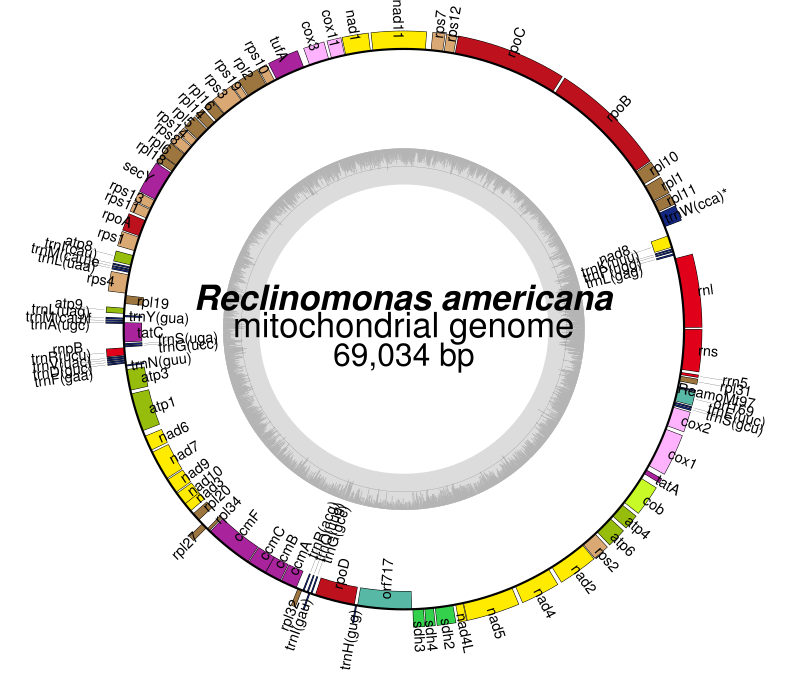
\includegraphics[width=\textwidth]{ogdraw-ra-mt.png} \\
      \hspace{1cm}
      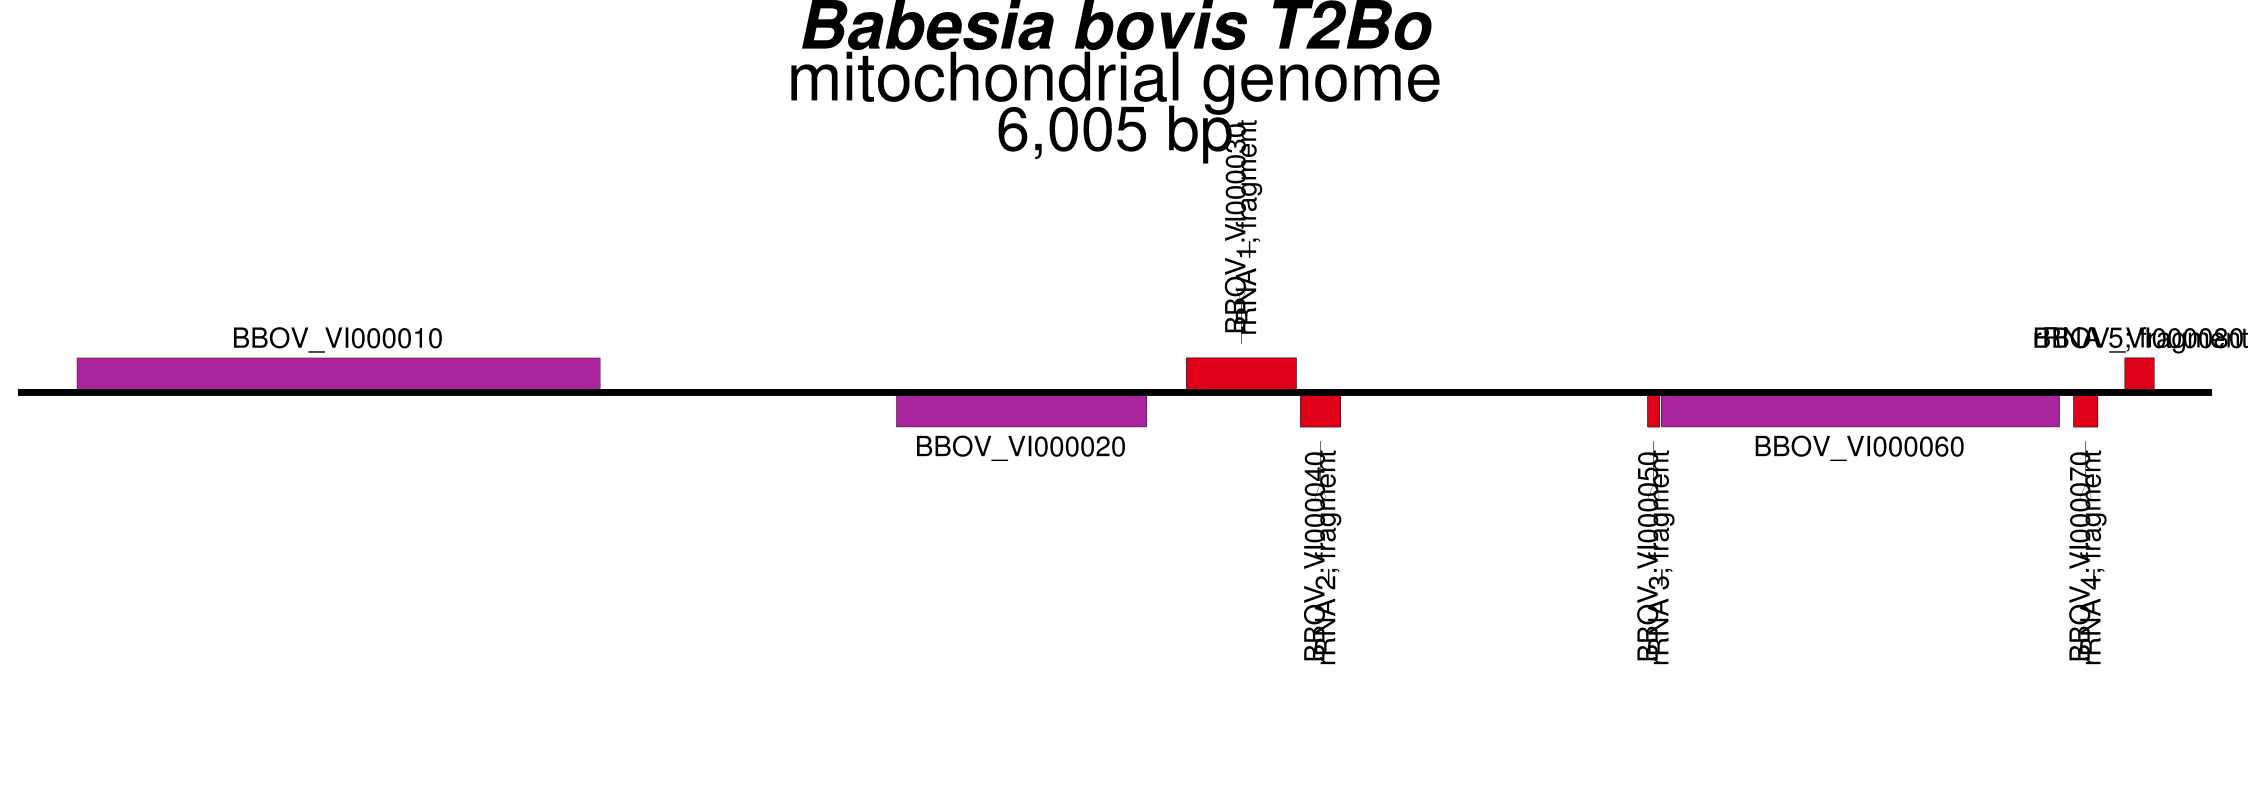
\includegraphics[width=\textwidth]{ogdraw-bb-mt.png} \\
      %\figcred{Figure credit: Sundararaman et al. PNAS 2013; OGMP; Tree of Life}
    \end{column}
  \end{columns}

\end{frame}

\begin{frame}{Cross-eukaryote mtDNA genome data assigns a `retention index' to mtDNA genes}
  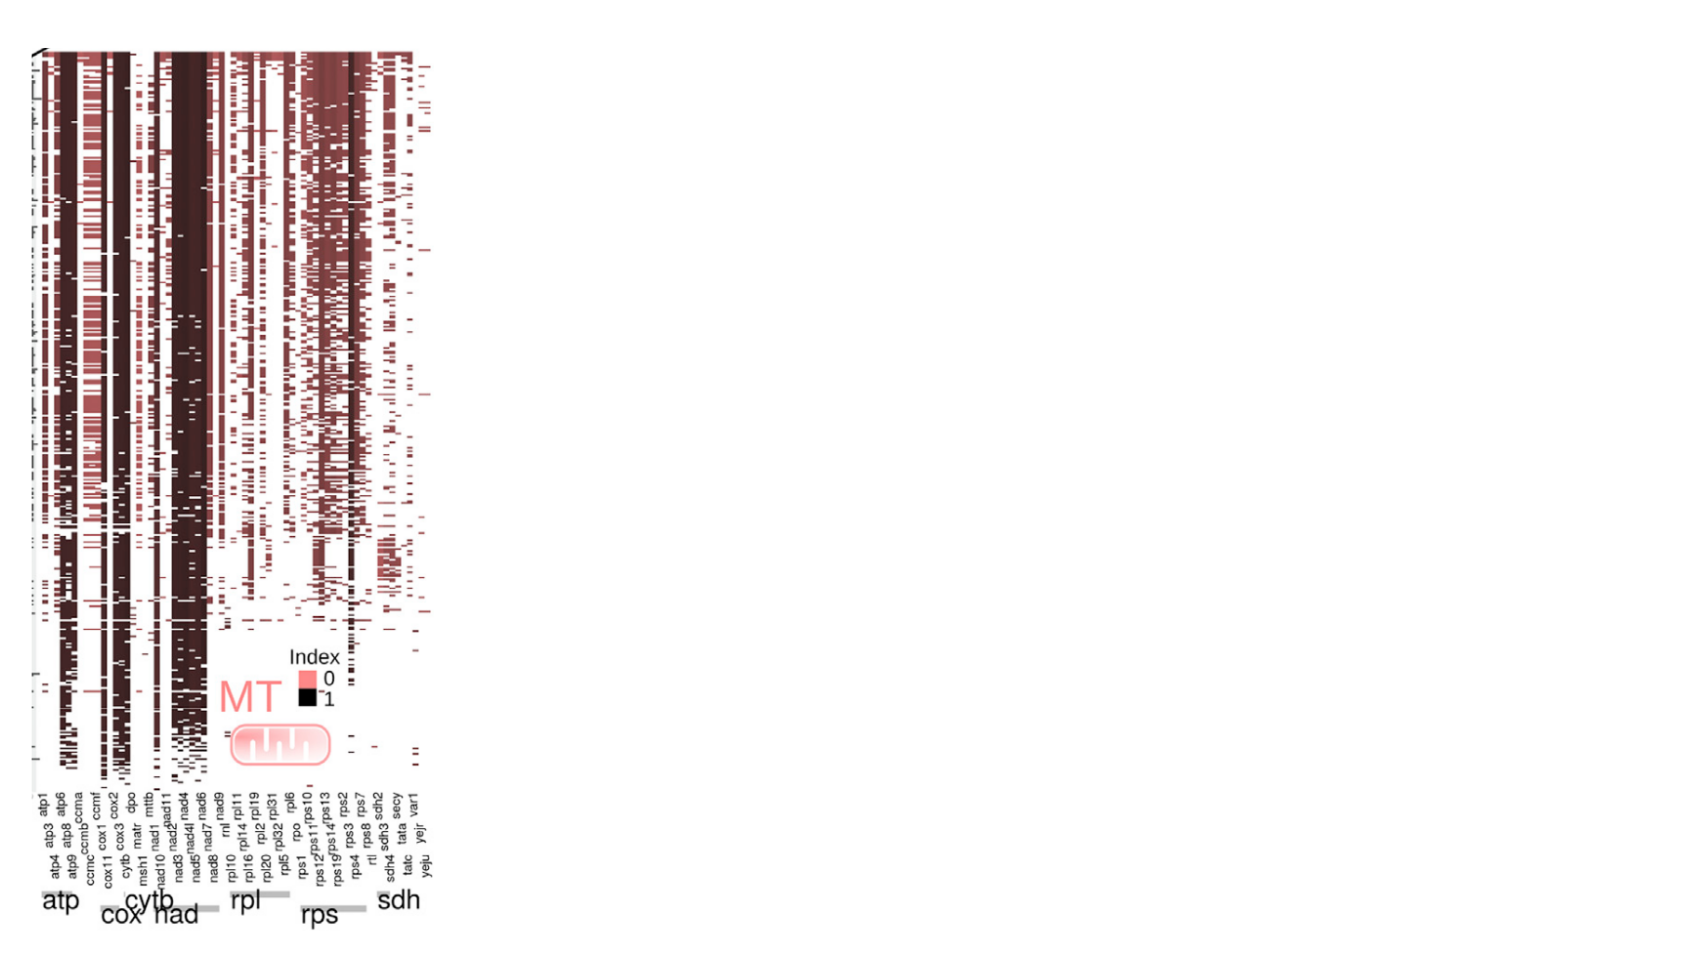
\includegraphics[width=1\textwidth]{wp1-slide1.png}
  \cellsys, \cellsystwo
\end{frame}
\begin{frame}{Cross-eukaryote mtDNA genome data assigns a `retention index' to mtDNA genes}
  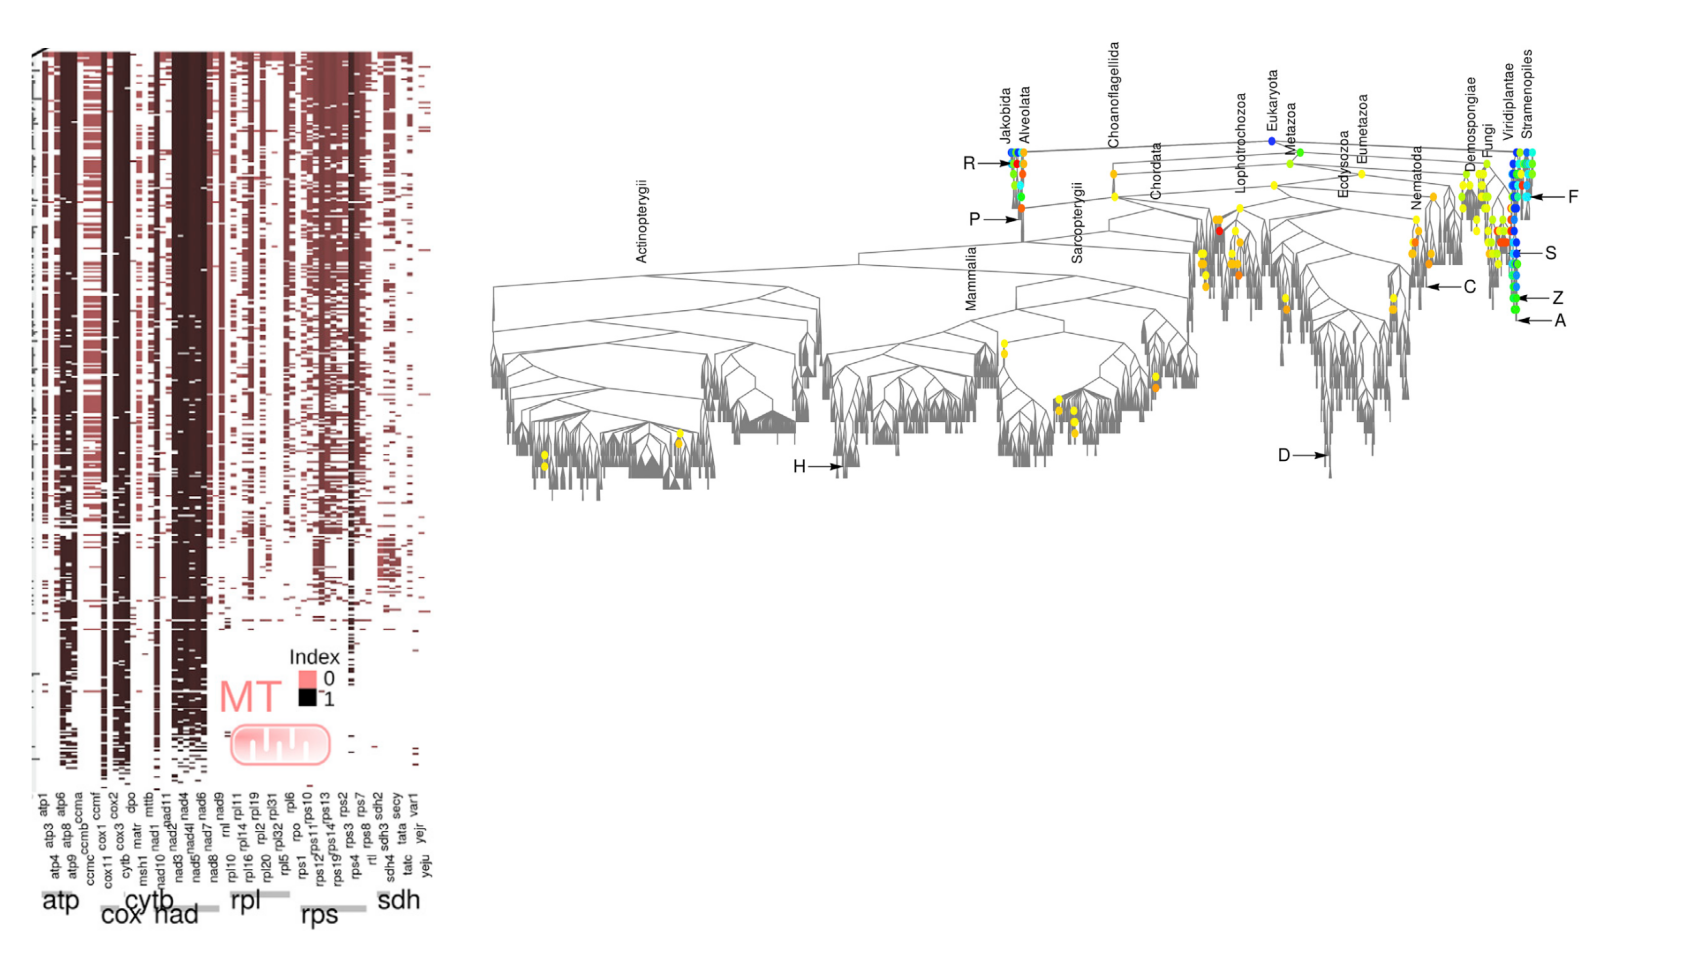
\includegraphics[width=1\textwidth]{wp1-slide2.png}
  \cellsys, \cellsystwo
\end{frame}
\begin{frame}{Cross-eukaryote mtDNA genome data assigns a `retention index' to mtDNA genes}
  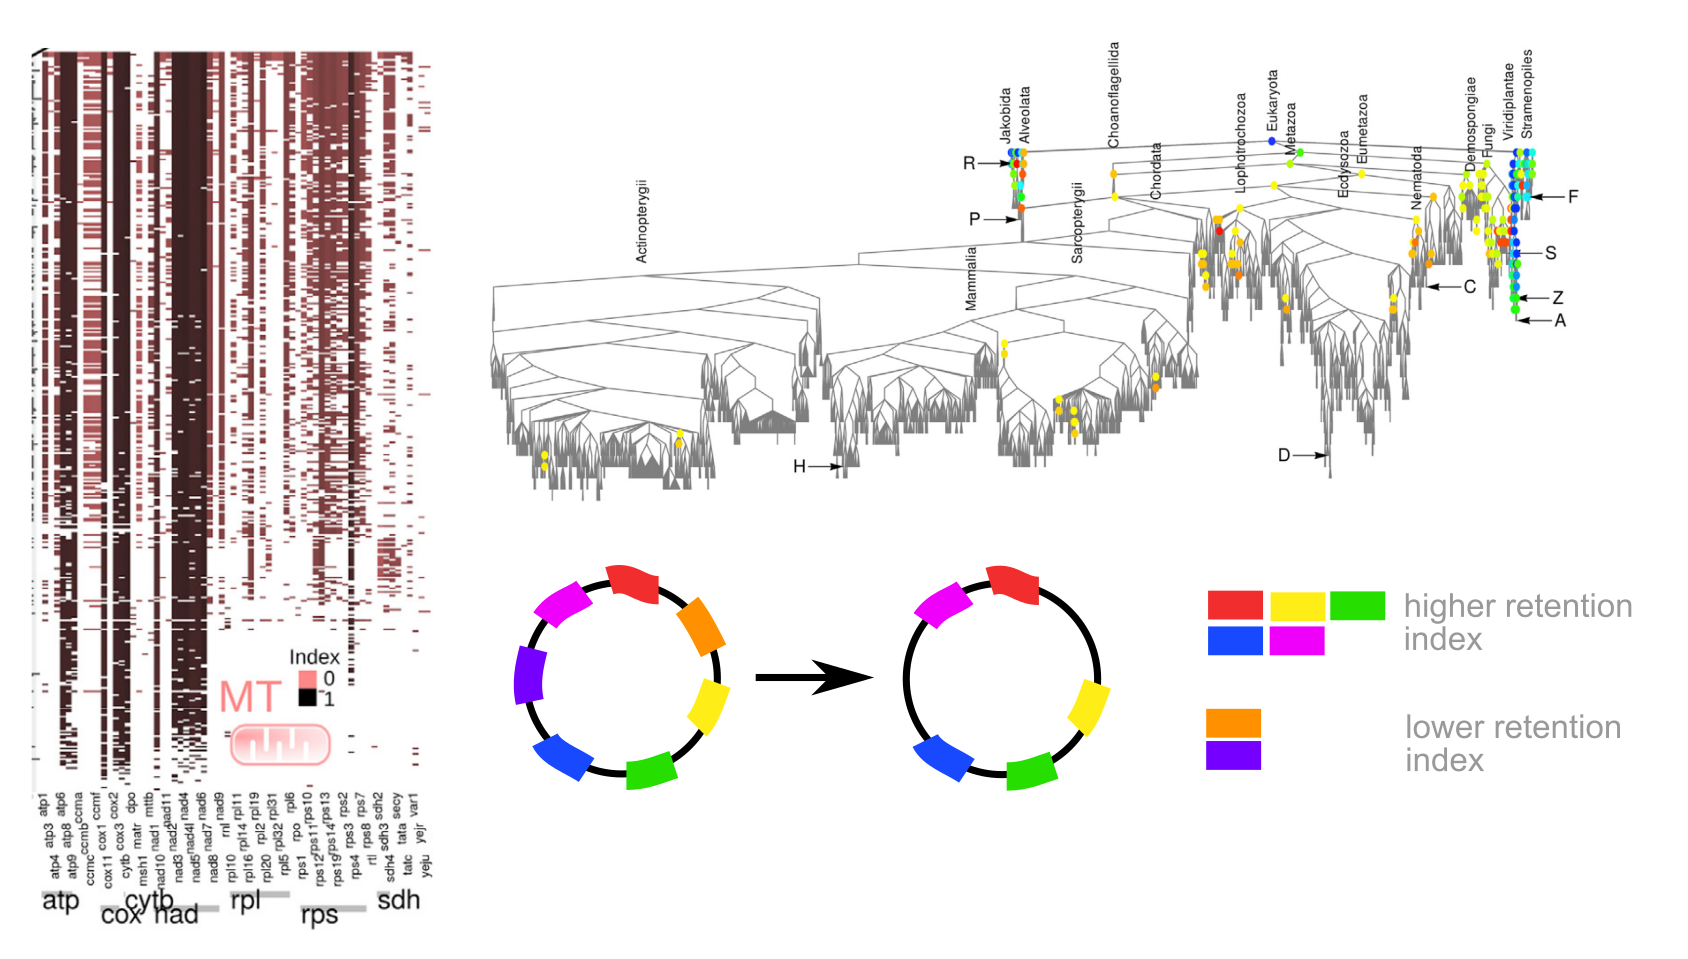
\includegraphics[width=1\textwidth]{wp1-slide3.png}
  \cellsys, \cellsystwo
\end{frame}
\begin{frame}{Hydrophobicity and energetic centrality (and others) predict gene-specific retention patterns}
  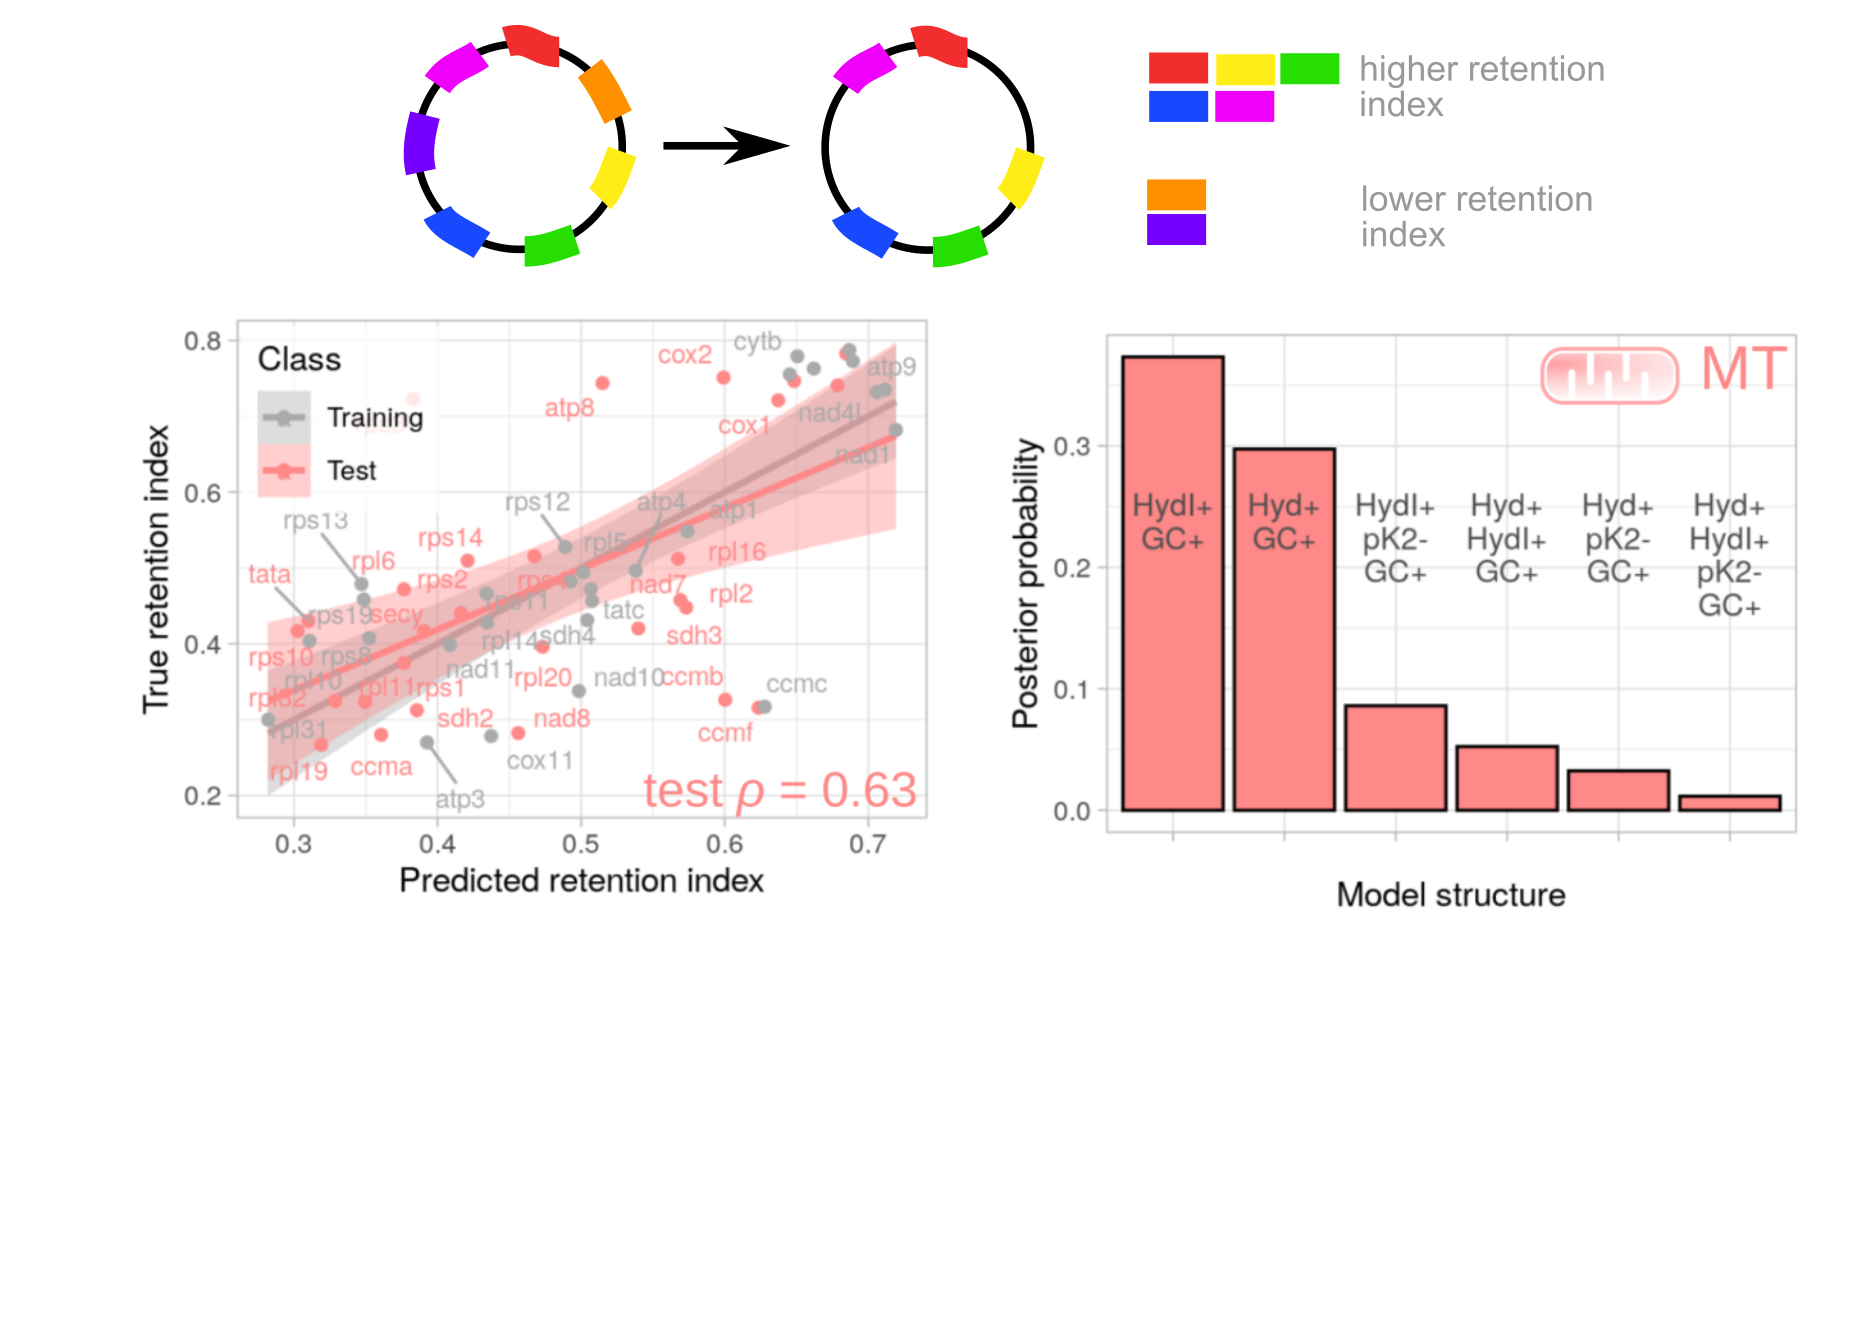
\includegraphics[width=.8\textwidth]{wp1-slide4.png}
  \cellsys, \cellsystwo
\end{frame}

\begin{frame}{mtDNA and cpDNA genome evolution are shaped by the same pressures}
  \hspace{-1cm}
        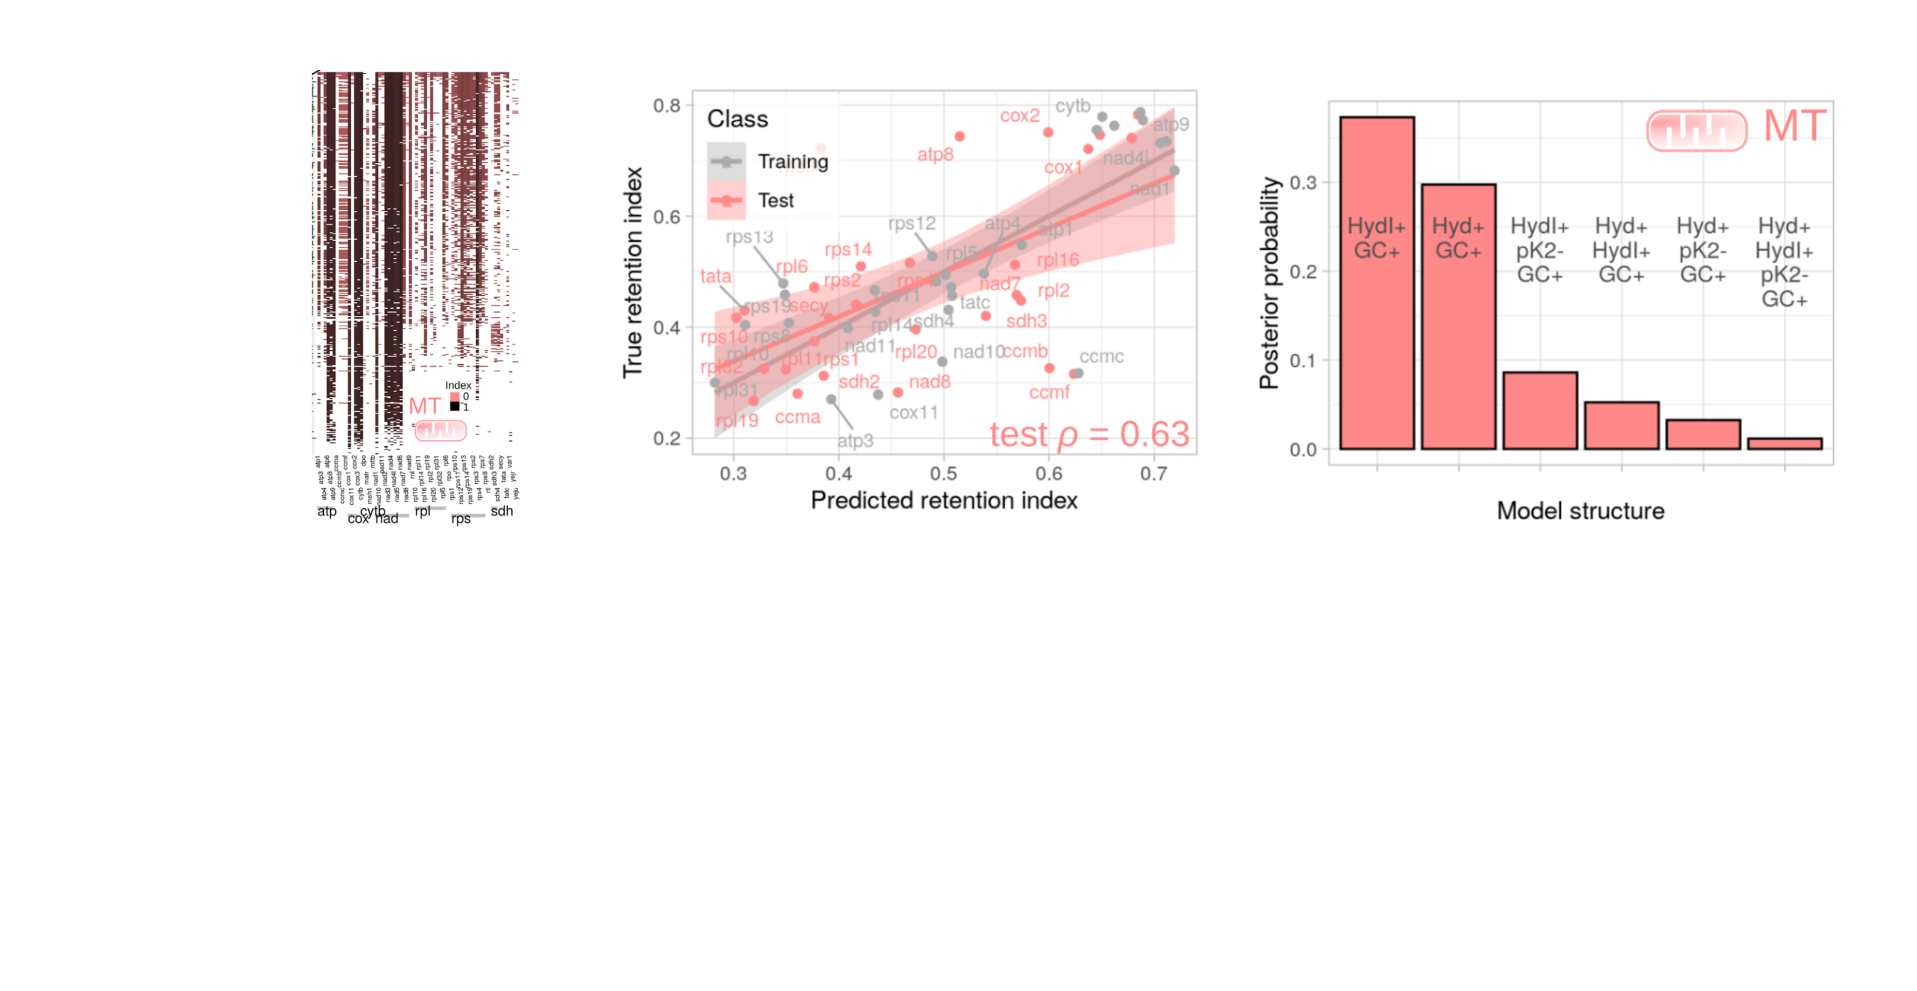
\includegraphics[width=1.1\textwidth]{uni-slide1.png} 
 
       \cellsystwo
\end{frame}
\begin{frame}{mtDNA and cpDNA genome evolution are shaped by the same pressures}
       \hspace{-1cm}
        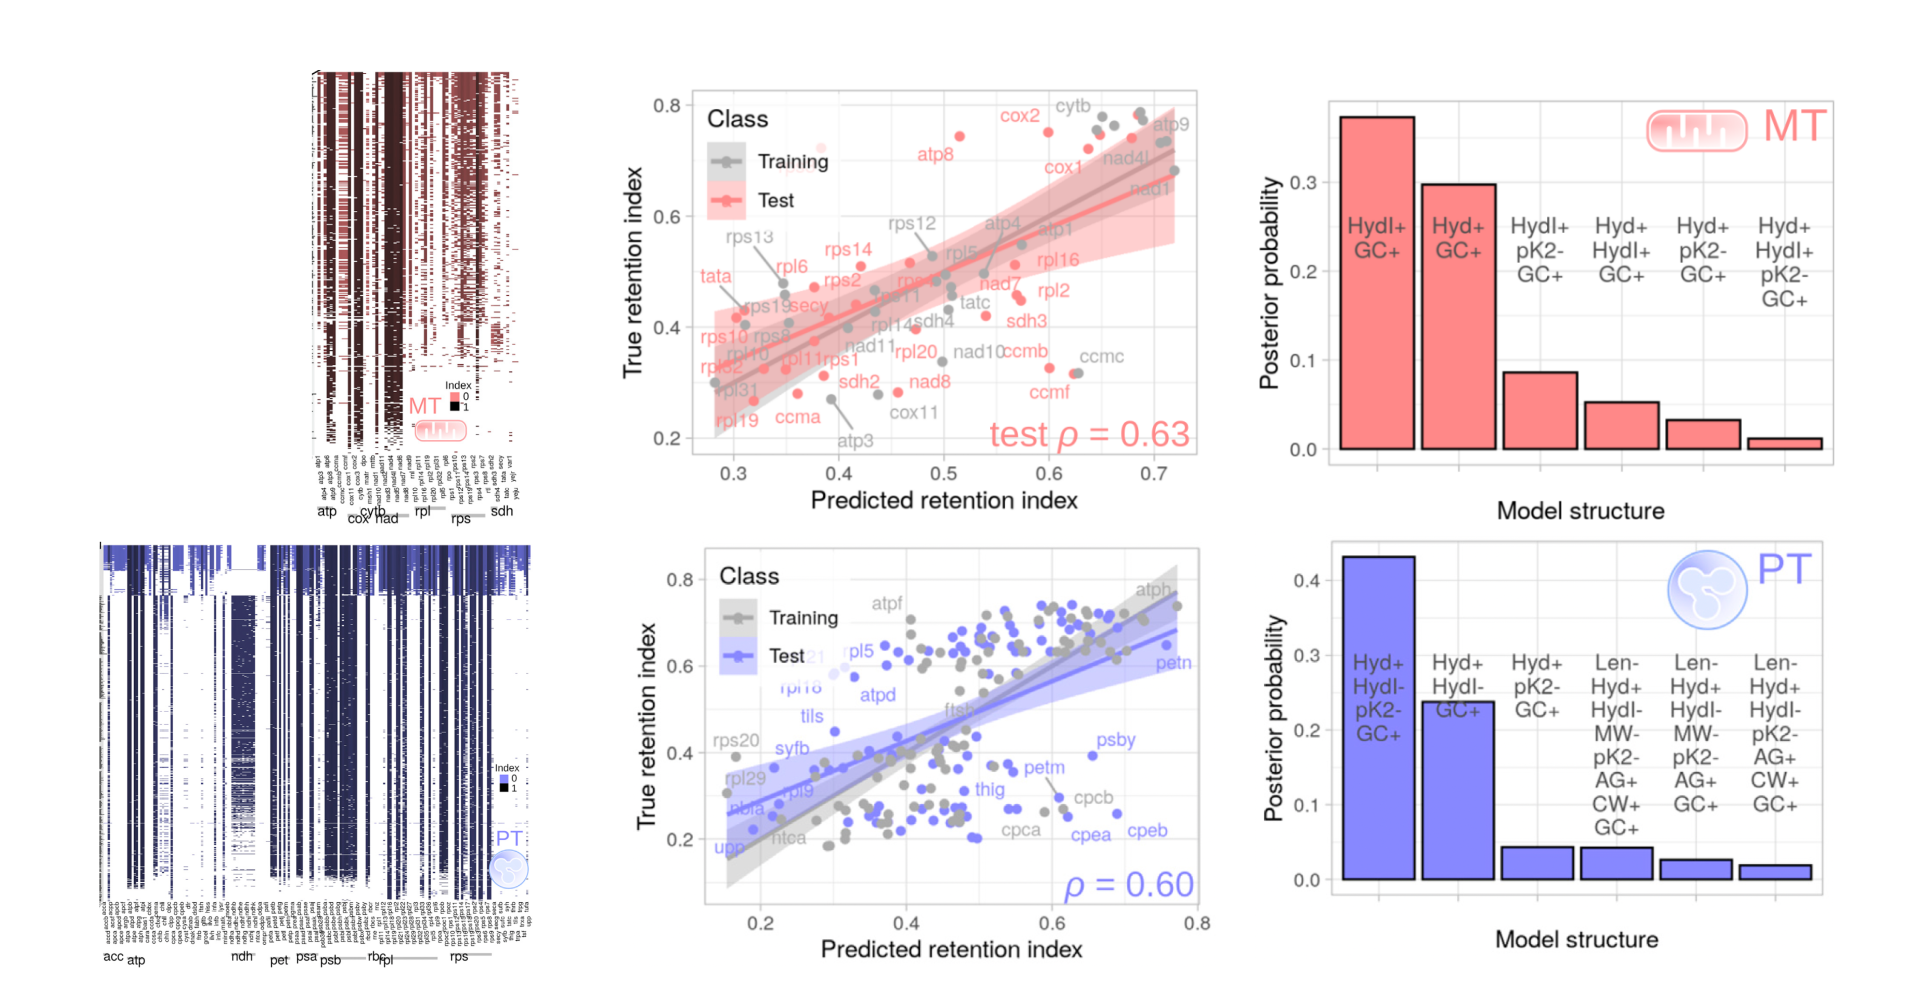
\includegraphics[width=1.1\textwidth]{uni-slide2.png} 
              \cellsystwo
\end{frame}
\begin{frame}{mtDNA and cpDNA genome evolution are shaped by the same pressures}
  \hspace{3cm}
  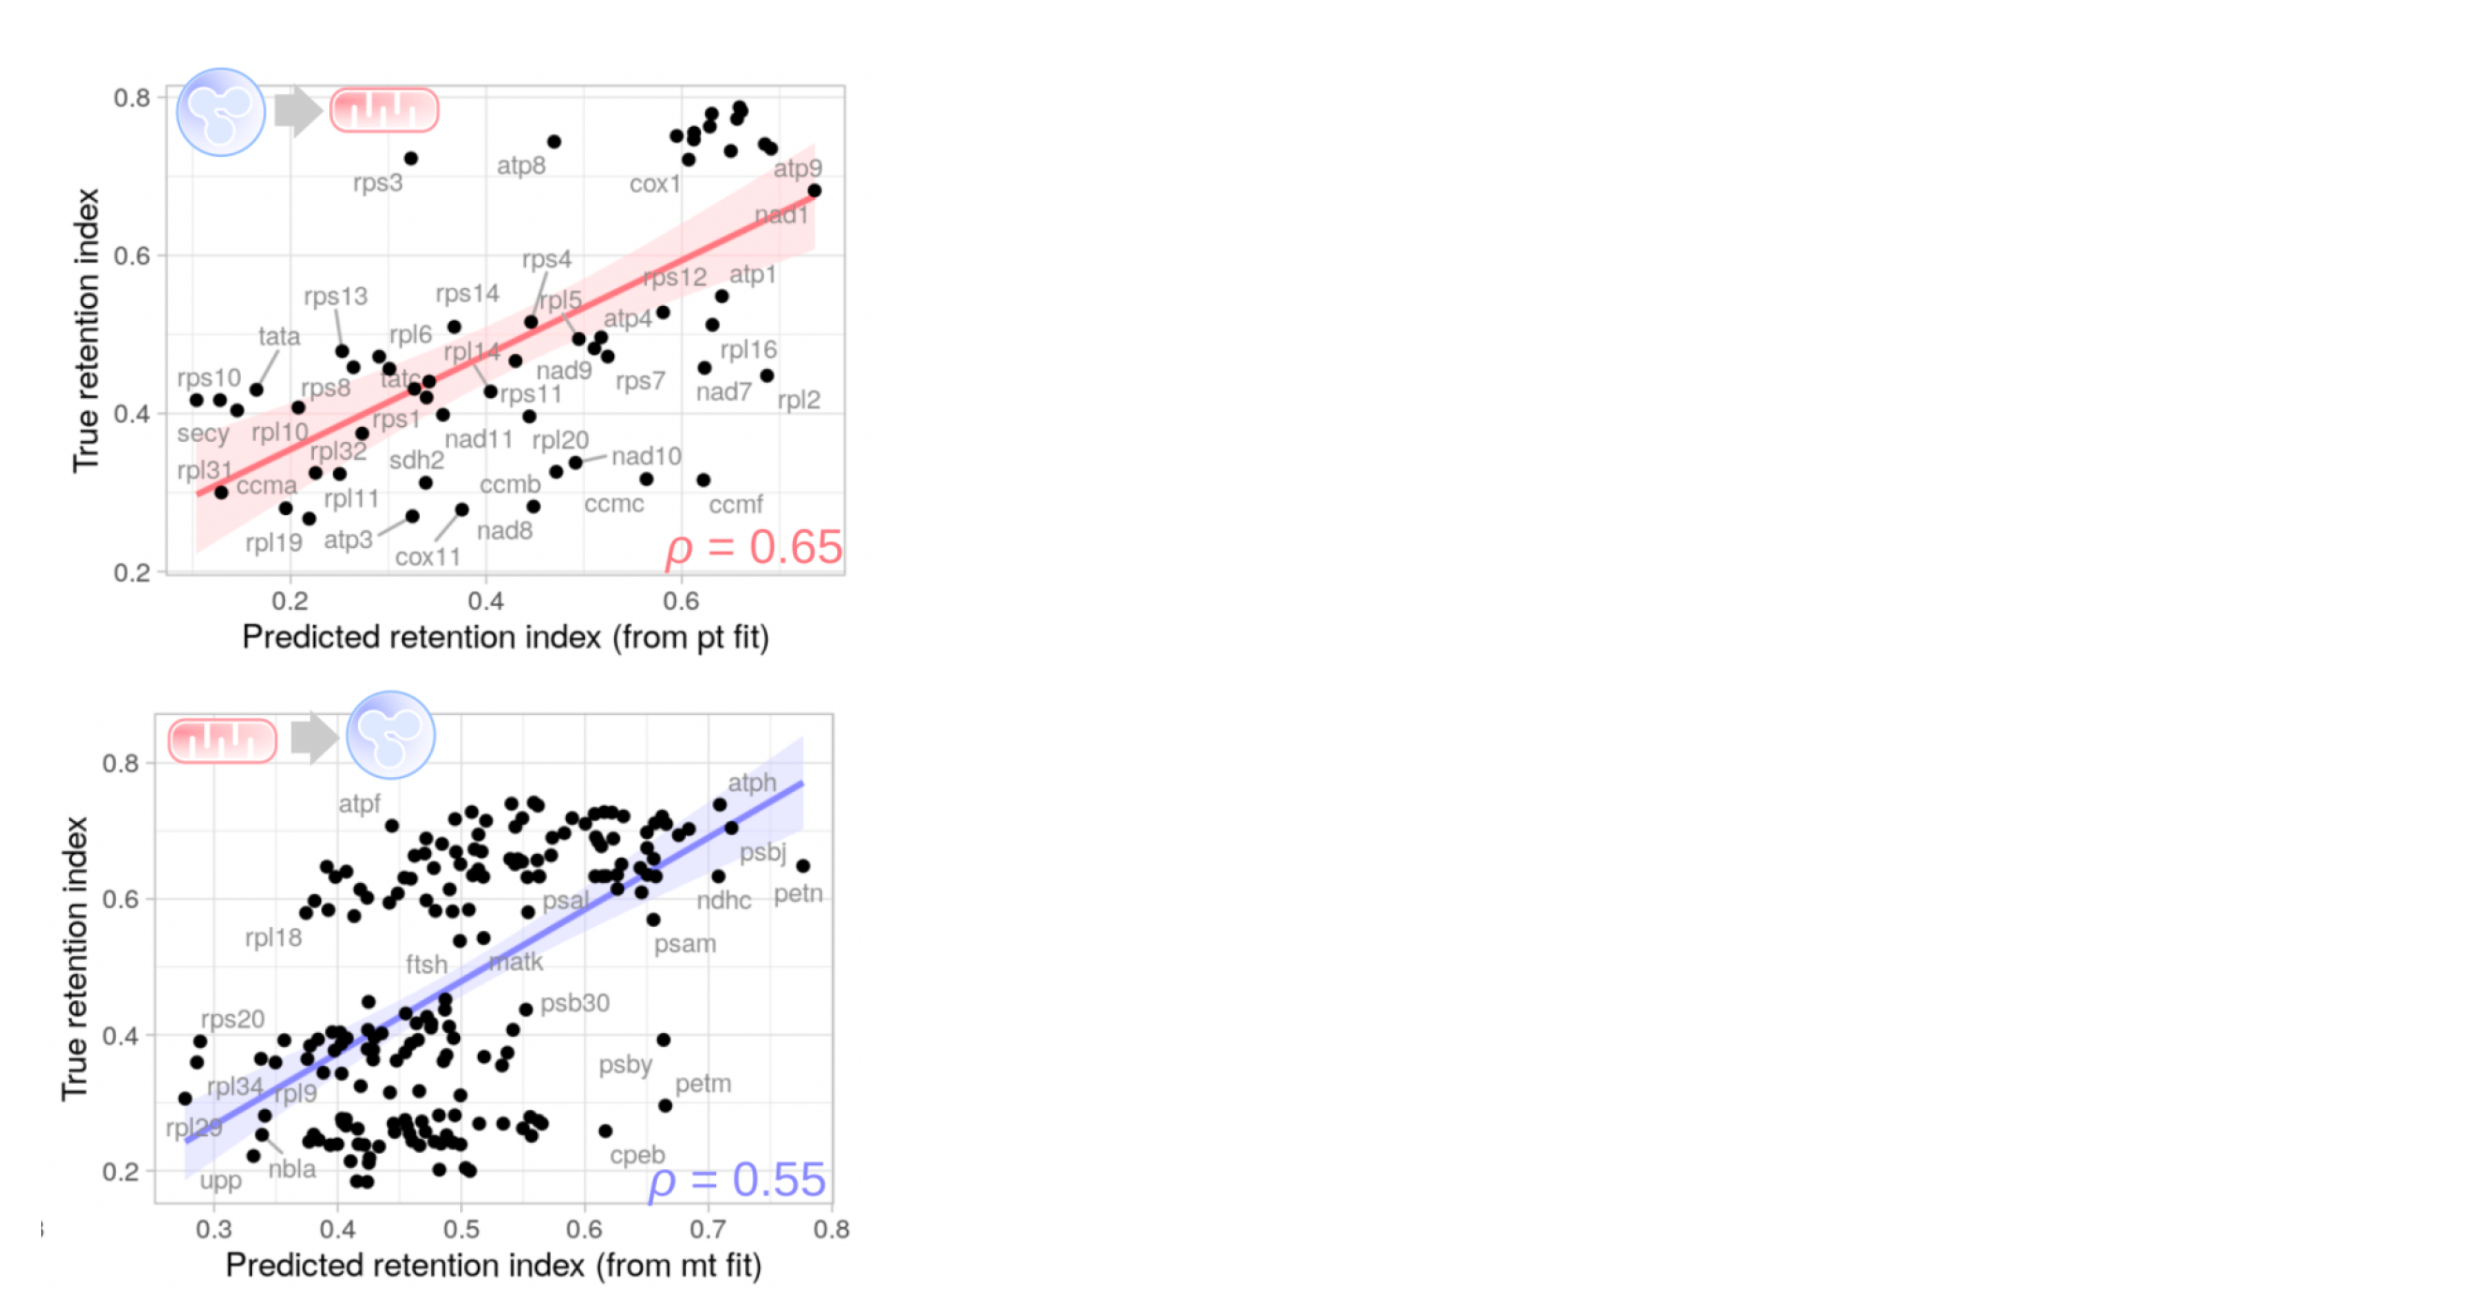
\includegraphics[width=\textwidth]{uni-slide9.png} 
              \cellsystwo
\end{frame}

\begin{frame}{Wrapping up -- Iain's uncensored opinions}
  \begin{itemize}
  \item If science is testing hypotheses with experiments, building and testing a single model is (borderline) not science
  \item Comparing different mechanistic models \textbf{is} science
  \item Statistics can do this with data and ideas alone, using frequentist (e.g. AIC) or Bayesian approaches
  \item Pros and cons to each: Iain thinks Bayes gives more breadth of interpretation, but requires some choices
  \item In R: AIC for simple models is fine in \texttt{base} R; \texttt{mombf} is good for Bayesian model selection; \texttt{rstanarm}, \texttt{BAS} and \texttt{BayesFactor} alternatives
  \item What did we miss? BIC; priors; LASSO, ridge, etc; any number of other approaches!
  \item Iain likes Mackay (2003) and Bishop (2006)
        \item Also -- most of applied stats -- hypothesis tests, regression, etc (STAT200!)

  \item Thanks, and let's chat! \includegraphics[width=0.025\textwidth]{twitter.png} \footnotesize @mitomaths
    \end{itemize}
\end{frame}


\begin{frame}{Tuberculosis}
  \begin{itemize}
  \item Tuberculosis causes millions of deaths worldwide
    \item TB is evolving resistance to drugs (4-20\% cases globally displaying multidrug resistance)
    \item Anti-microbial resistance (AMR) is UN's \#1 global societal challenge, anticipated to cause 10m deaths and cost \$100trn by 2050
      \end{itemize}
  \centering
    \includegraphics[width=.6\textwidth]{tb-bacterium.jpg} \\
\figcred{Figure source: 123RF}
\end{frame}

\begin{frame}{Tuberculosis evolution}
 \begin{itemize}
 \item Casali \emph{et al.}: 1000 TB isolates from Russia sequenced
 \item Mutations conferring resistance to different drugs characterised
   \end{itemize}
  \centering
    \includegraphics[width=.7\textwidth]{casali-tb.png} \\
\casali
\end{frame}
 
\begin{frame}{HyperTraPS infers pathways of AMR evolution in TB}
  \centering
    \includegraphics[width=.9\textwidth]{tb-3.png} \\
\hypertraps, \marcus
\end{frame}

\begin{frame}{HyperTraPS infers pathways of AMR evolution in TB}
   \begin{itemize}
   \item Consistent early dynamics, more heterogeneous later
   \item Which drug has highest probability of future resistance acquisition, given current state?
     \item What demographic / geographical features influence evolutionary pathways?
     \end{itemize}
  \centering
    \includegraphics[width=.45\textwidth]{tb-3.png}     \includegraphics[width=.5\textwidth]{tb-4.png} \\
\hypertraps, \marcus
\end{frame}

\section{Malaria progression}

\begin{frame}{Malaria progression}
  \begin{itemize}
  \item Severe malaria kills $>400k$ a year, mainly African children
  \item WHO treatment guidelines are coarse-grained `one size fits all'
    \item These guidelines don't capture patient and disease heterogeneity
  \end{itemize}
  \vspace{1cm}
  \centering
  \includegraphics[width=\textwidth]{npj-banner.png} \\
  \jallow, \malaria
\end{frame}

\begin{frame}{HyperTraPS can be applied to learn pathways of symptom acquisition in malaria}
        \begin{itemize}
        \item Diverse clinical features can be coded as presence or absence
\item 2904 Gambian children admitted to hospital: incomplete records
        \end{itemize}
        \centering
          \includegraphics[width=.6\textwidth]{malaria-data1.png} \\
 \jallow, \malaria
\end{frame}

\begin{frame}{HyperTraPS can be applied to learn pathways of symptom acquisition in malaria}
  \begin{itemize}
  \item HyperTraPS learns probabilities of symptom orderings in patients that survived/died
    \item Ordering without longitudinal data
  \end{itemize}
  \centering
\includegraphics[width=.75\textwidth]{malaria-map.png} \\
\malaria
\end{frame}



\begin{frame}{HyperTraPS reveals pathways and patient risks in malaria}
  \begin{columns}
    \begin{column}{0.3\textwidth}
  \begin{itemize}
  \item Risk markers: symptoms that appear at different stages in surviving/dead patients
    \item Only `first order' -- we can do better
    \end{itemize}
    \end{column}
    \begin{column}{0.7\textwidth}
  \includegraphics[width=\textwidth]{malaria-distns.png}\\
  \malaria
    \end{column}
  \end{columns}
  
\end{frame}


\begin{frame}{HyperTraPS predicts hidden symptoms, future behaviour, and prognoses}
  \begin{columns}
    \begin{column}{0.5\textwidth}
  \begin{itemize}
  \item Training-test split: learn pathways from training data, ask how likely a test observation is to be on a `death' pathway
    \item Accounts for all observed features and any learned interactions
  \end{itemize}
    \end{column}
    \begin{column}{0.5\textwidth}
      \includegraphics[width=\textwidth]{malaria-risk1.png}
    \end{column}
  \end{columns}
\malaria
\end{frame}

\begin{frame}{HyperTraPS predicts hidden symptoms, future behaviour, and prognoses}
  \begin{columns}
    \begin{column}{0.5\textwidth}
  \begin{itemize}
  \item Training-test split: learn pathways from training data, ask how likely a test observation is to be on a `death' pathway
    \item Accounts for all observed features and any learned interactions
    \item 81\% classifications successful, false negative rate 6\%
  \end{itemize}
    \end{column}
    \begin{column}{0.5\textwidth}
      \includegraphics[width=\textwidth]{malaria-risk2.png}
    \end{column}
  \end{columns}
\malaria
\end{frame}



\begin{frame}{HyperTraPS predicts hidden symptoms, future behaviour, and prognoses}
  \begin{columns}
    \begin{column}{0.3\textwidth} 
  \begin{itemize}
  \item Split data into 50\% training, 50\% test
  \item Hide 10\% of features in test set
  \item Symptoms recovered with 83\% success
  \end{itemize}
    \end{column}
    \begin{column}{0.7\textwidth}
\includegraphics[width=\textwidth]{malaria-predict1.png} \\
\malaria
    \end{column}
  \end{columns}
\end{frame}



\end{document}
